

\chapter{Hydrodynamic interactions between two colloids near a wall}
%%%%%%%%%%%%%%%%%%%%%%%%%%%%%%%%%%%%%%%%%%%%%%%%%%%%%%%%%%%%%%%%%%%%%%%%%%%%%%%%%%%%%%%%%%%%%%%%%%%%%%%%%%%%%%%%%%%%%%%%%%%%%%%%%%%%%%%%%%%%%%%%%%%%%%%%%%%%%%%%%%%%%%%%%%%%%%%%%%%%%%%%%%%%%%%%
\section{Introduction} 

The last chapter focuses on a very simple, ideal case. The colloid is away from any confinement. Thought we mention Brownian solutes, we consider each colloid in the solute as non-interacting with its peers. These assumptions and choices are strong, and very often in biological settings, they do not appropriately describe the dynamics of the system. Fortunately, and perhaps out of necessity, confined Brownian motion has been extensively investigated over the last century. Even at long range, hydrodynamic interactions influence behaviour of colloids diffusing in a fluid ~\cite{kim_microhydrodynamics_2005, Batchelor_1976}. We now know that introducing a single, infinite boundary near a colloid effectively increases the fluid's viscosity in an inhomogeneous and anisotropic way, differenciating in two separate modes the motions along the boundary direction, and perpendicular to it ~\cite{brenner_slow_1961}. In turn, because the diffusion coefficient inversely depends on the viscosity felt by the colloid (Eq.~\ref{Eq:Stokes-einstein}), it is hindered by rigid confinement. Moreover, volume dfraction also hinders a tagged colloid's diffusion, while collective diffusion of the solute speeds up as osmotic pressure gradients become stronger with higher local concentration~\cite{Batchelor_1976}. The pair diffusion of colloids in hydrodynamic interactions is thoroughly documented ~\cite{JeffreyOnishi1984, JeffreyOnishi1984a}.

It is fairly common, in nature, to find highly confined solutions of high volume dfraction, that is to say, occupied volume by the colloids compared to total volume. For instance, the cell cytoplasm is packed with proteins, RNA, ribosomes, organelles, etc., and confined by a cell membrane. A question thus arises: ``How do crowding and confinement couple hydrodynamically?''. This coupling is difficult to resolve for any intercolloidal distance at any distance from confinement. Indeed, it is permitted only to a certain extent to simply superimpose the contributions from the confinement and the crowding. This chapter aims at first decomposing the problem into confined, dilute suspensions, then pair diffusion. Then, I move to the coupling of these two effects, and developments used to model this coupling. I present an experimental study carried out by Dufresne \emph{et al.}~\cite{Dufresne_2000} exploring the effect on confinement on pair diffusion and recover these results numerically. Finally, I present some prospective work on going beyond Dufresne's study numerically and experimentally.


\begin{figure}
    \centering
    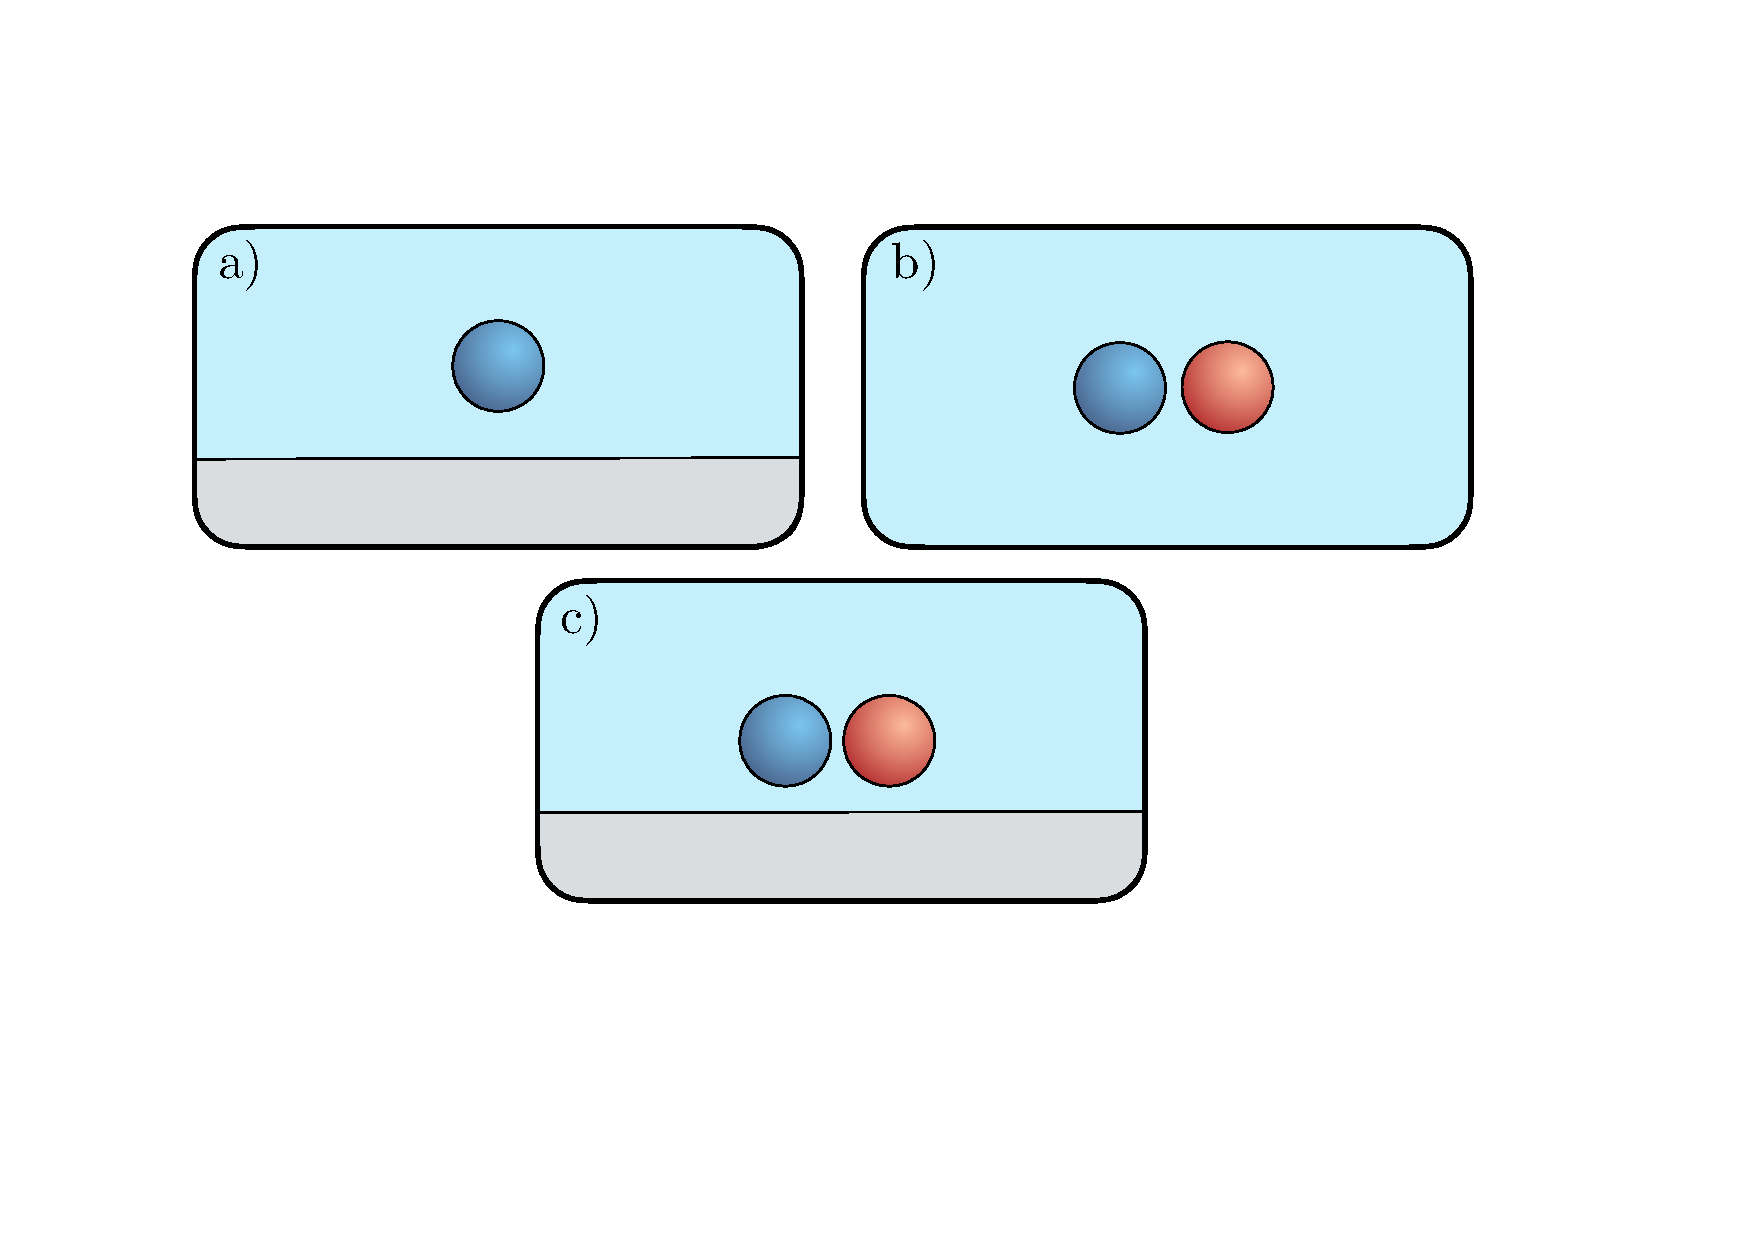
\includegraphics[width=0.8\textwidth]{figures/chapter2/intro.pdf}
    \caption[Schematic of wall-colloid and colloid-colloid lubrications.]{Schematic representation of the three cases of interest for this chapter. $a)$ A single colloid diffusing in a fluid over an infinite, hard boundary. $b)$ Two colloids interacting with each other through hydrodynamic interactions in an unbounded fluid. $c)$ A combination of the two first cases, where two colloids interact with each other and with an infinite, hard boundary. }
    \label{intro}

\end{figure}


\section{Interactions between a colloid and a wall}

I describe here all interactions that occur in an experimental setup of a silica colloid in a fluid near a silica plate. We take the plate normal to the vertical $z$ axis, laying at $z=0$. Over that plane is a fluid of density $\rho$, viscosity $\eta$, and thermal energy $k_\mathrm{B} \Theta$ with $k_\mathrm{B}$ the Boltzmann constant. All parameters for the upcoming derivations are summarised in Table~\ref{tab:physical_parameters}.
\begin{figure}
    \centering
    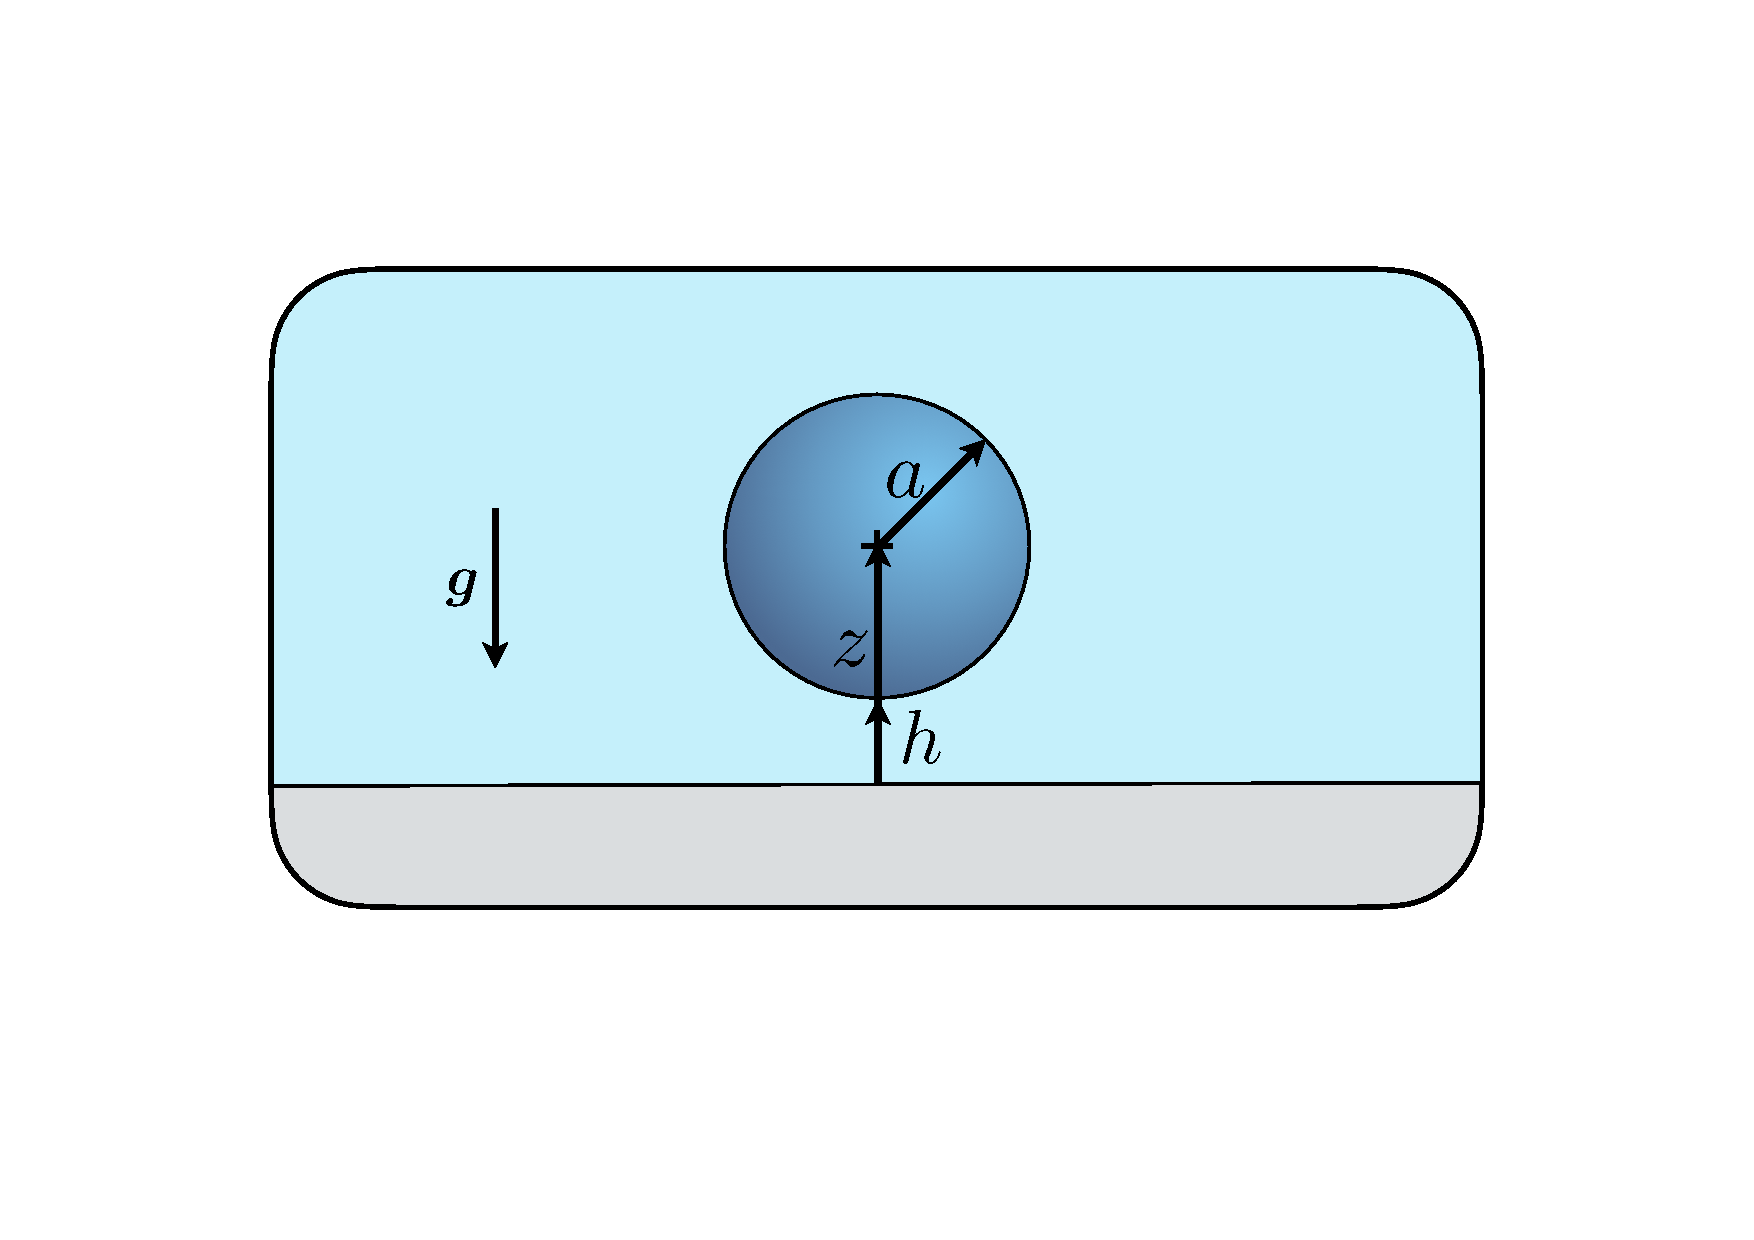
\includegraphics[width=.5\textwidth]{figures/chapter2/bead_plate.pdf}
    \caption[Schematic of a colloid diffusing over a hard wall.]{Schematic representation of a colloid of radius $a$ at a distance $z$ from an infinite plane.}
    \label{System_beadplate}
\end{figure}
In the fluid, we now submerge a colloidal silica particle of radius $a$, of the micron scale. Due to the no-slip boundary conditions at contact with the plane and the colloid's surfaces, we must modify the effective viscosity of the fluid as the colloid evolves in the $z$ direction. This correction brings not only inhomogeneity along the $z$-axis but also anisotropy, as the $x$ and $y$ components of the friction coefficient differ from the $z$ component.
\begin{table}[h]
\centering
\caption{Typical parameters for a silica colloid suspended in water near a silica wall at room temperature. Values are indicative.}
\label{tab:physical_parameters}
\begin{tabular}{llll}
\hline
Symbol & Quantity & Typical value \\
\hline
$a$ & Colloid radius & $0.5 - 2$ $\upmu \mathrm{m}$ \\
$z$ & Distance from wall centre-to-wall $a - 20a$ & $\upmu \mathrm{m}$ \\
\hline
$\rho$ & Water density & $10^3$ $\mathrm{kg.}\mathrm{m}^{-3}$ \\
$\eta$ & Water viscosity & $10^{-3}$ $\mathrm{Pa.}\mathrm{s}$ \\
\hline
$\Theta$ & Temperature & $298$ $\mathrm{K}$ \\
$k_\mathrm{B}$ & Boltzmann constant & $1.38\times10^{-23}$ $\mathrm{J}.\mathrm{K}^{-1}$ \\
$k_\mathrm{B}\Theta$ & Thermal energy & $4.1\times10^{-21}$  $\mathrm{J}$ \\
\hline
$\eta_\perp(z)$ & Effective perpendicular viscosity & $\eta$ to $\gg\eta$  \\
$\eta_\parallel(z)$ & Effective parallel viscosity & $\eta$ to $\gg\eta$  \\
\hline
$l_\mathrm{B}$ & Boltzmann length & $0.1 - 10$ $\upmu \mathrm{m}$ \\
$l_\mathrm{D}$ & Debye length & $1 - 100$ $\mathrm{nm}$ \\
\end{tabular}
\end{table}


\subsection{Modified effective viscosity}
In his seminal work~\cite{brenner_slow_1961}, Brenner derived the exact expression for the effective viscosity felt by a sphere moving perpendicularly to a plane wall, $\eta_\perp(z)$, as:
\begin{equation}
    \label{Brenner}
    \eta_\perp (z) = \dfrac{4}{3} \eta  \sinh(\alpha) \sum_{n=1}^{\infty} \dfrac{n(n+1)}{(2n-1)(2n+3)} \left\{ \dfrac{2 \sinh[(2n+1)\alpha] + (2n+1) \sinh(2\alpha)}{4 \sinh^2[(n+\dfrac{1}{2})\alpha] - (2n+1)^2 \sinh^2(\alpha)} - 1 \right\}~,
\end{equation}
with $\alpha = \cosh^{-1} \left[ (z+a)/a \right]$. Because Brenner obtained the effective viscosity from solving the full Stokes equations with a no-slip boundary condition at the wall, it is worth noting that this expression is exact and valid for all values of $z/a > 0$, that is to say up until colloid/plane contact. However, for the sake of efficient numerical computations later on, we avoid infinite-series computations and prefer the use of Pad\'e approximants ~\cite{BakerGravesMorris_1996}, which were used by Honig ~\cite{Honig_1971}, Bevan and Prieve ~\cite{Bevan_2000} to approximate Brenner's result as:
\begin{equation}
    \label{Padé}
    \eta_\perp (z) \simeq \eta \dfrac{6z^2 + 2az}{6z^2 - 9az + 2a^2}~.
\end{equation}
The parallel effective viscosity, on the other hand, was derived by Fax\'en ~\cite{Faxen_1924} for $z/a > 0.1$ and is given by the following expression:
\begin{equation}
    \eta_\parallel (z) \simeq  \dfrac{\eta}{1 - \dfrac{9}{16} \dfrac{a}{z} + \dfrac{1}{8} \left( \dfrac{a}{z} \right)^3 - \dfrac{45}{256} \left( \dfrac{a}{z} \right)^4 - \dfrac{1}{16} \left( \dfrac{a}{z} \right)^5}~.
    \label{Faxén}
\end{equation}


\begin{figure}
    \centering
    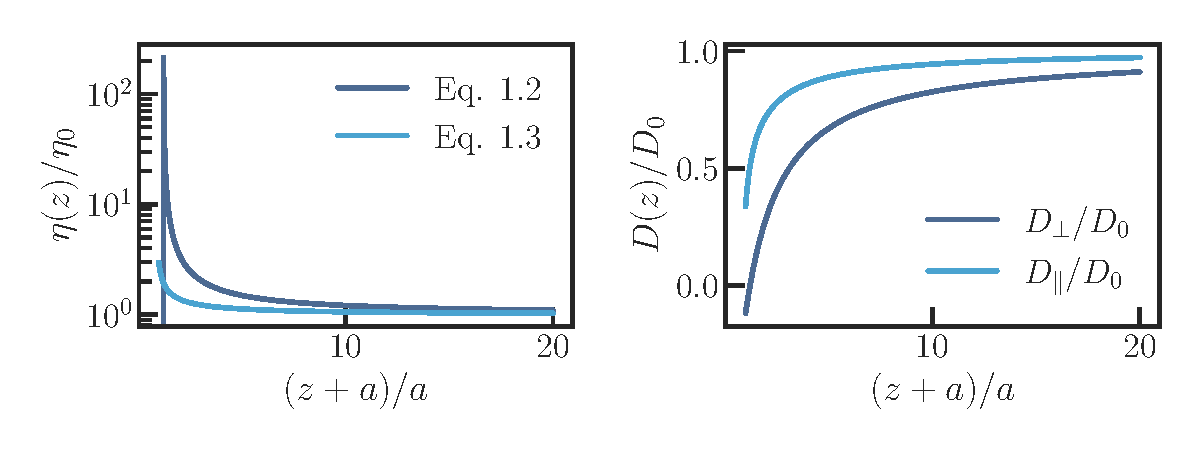
\includegraphics[width=1\textwidth]{figures/chapter2/diffusion_coefficients_brenpad.pdf}
    \caption[Effective viscosities and corresponding effective colloid diffusion coefficients corrected by interactions with the wall.]{Effective viscosities and corresponding effective diffusion coefficients for a colloid diffusing over a plane. Left panel: Effective viscosities $\eta_\perp$ (navy) and $\eta_\parallel$ (sky blue) renormalised by the bulk viscosity $\eta_0$ as a function of the distance to the wall $z$. Right panel: Effective diffusion coefficients $D_\perp$ (navy) and $D_\parallel$ (sky blue) renormalised by the bulk diffusion coefficient $D_0$ as a function of the renormalised colloid center-to-wall distance $(z+a)/a$.}
    \label{Figdperdpar}

\end{figure}
Both Eq.~\ref{Padé} and Eq.~\ref{Faxén} demonstrate that the viscosity effectively increases as the colloid approaches the wall (Left panel of Fig. \ref{Figdperdpar}). In turn, the effective diffusion coefficients decrease (Right panel of Fig.~\ref{Figdperdpar}). Furthermore, these expressions can be used to simulate the Brownian motion of a colloid over a plane up until contact. We note that in the limit of $z/a \to 1$, $\eta_\perp$ captures the divergence close to the wall. This is an expected behaviour; as the colloid approaches the wall, the fluid in between is squeezed out and the lubrication forces diverge. However, $\eta_\parallel$ does not capture the weak logarithmic divergence expected as the surface-to-surface gap tends to zero. Other means of accurately capturing the divergence exist, which I mention down below. 

\subsection{Total potential}

Furthermore, in order to write the correct overdamped Langevin equation for a simulation, we recall that the colloid is also subject to a number of forces, which we now carefully enumerate as they will be present throughout the remainder parts of this chapter.


\subsubsection{Gravitational potential and buoyant mass}
We express the gravitational potential acting upon the colloid as:
\begin{align}
    U_\mathrm{grav} &  = \Delta m g z~,\\
    & = \dfrac{4}{3} \pi a^3 (\rho_\mathrm{colloid} - \rho_\mathrm{fluid}) g z~,
    \label{grav_potential}
\end{align}
where $\Delta m$ is the buoyant mass of the colloid, $g$ is the acceleration of gravity, and $\rho_\mathrm{colloid}$ and $\rho_\mathrm{fluid}$ are the mass densities of the colloid and the fluid, respectively.
We may rewrite the above Eq.~\ref{grav_potential} as:
\begin{equation}
U_\mathrm{grav} = \dfrac{k_\mathrm{B} \Theta}{l_\mathrm{B}} z~,
\label{grav_potential_lB}
\end{equation}
where $l_\mathrm{B}$ is Boltzmann's length, defined as $l_\mathrm{B} = (k_\mathrm{B} \Theta)(g\Delta m )$. Boltzmann's length quantifies the distance over which gravitational potential energy is comparable to thermal energy.



\subsubsection{Electrostatic potential and double-layer interactions}
\begin{figure}
    \centering
    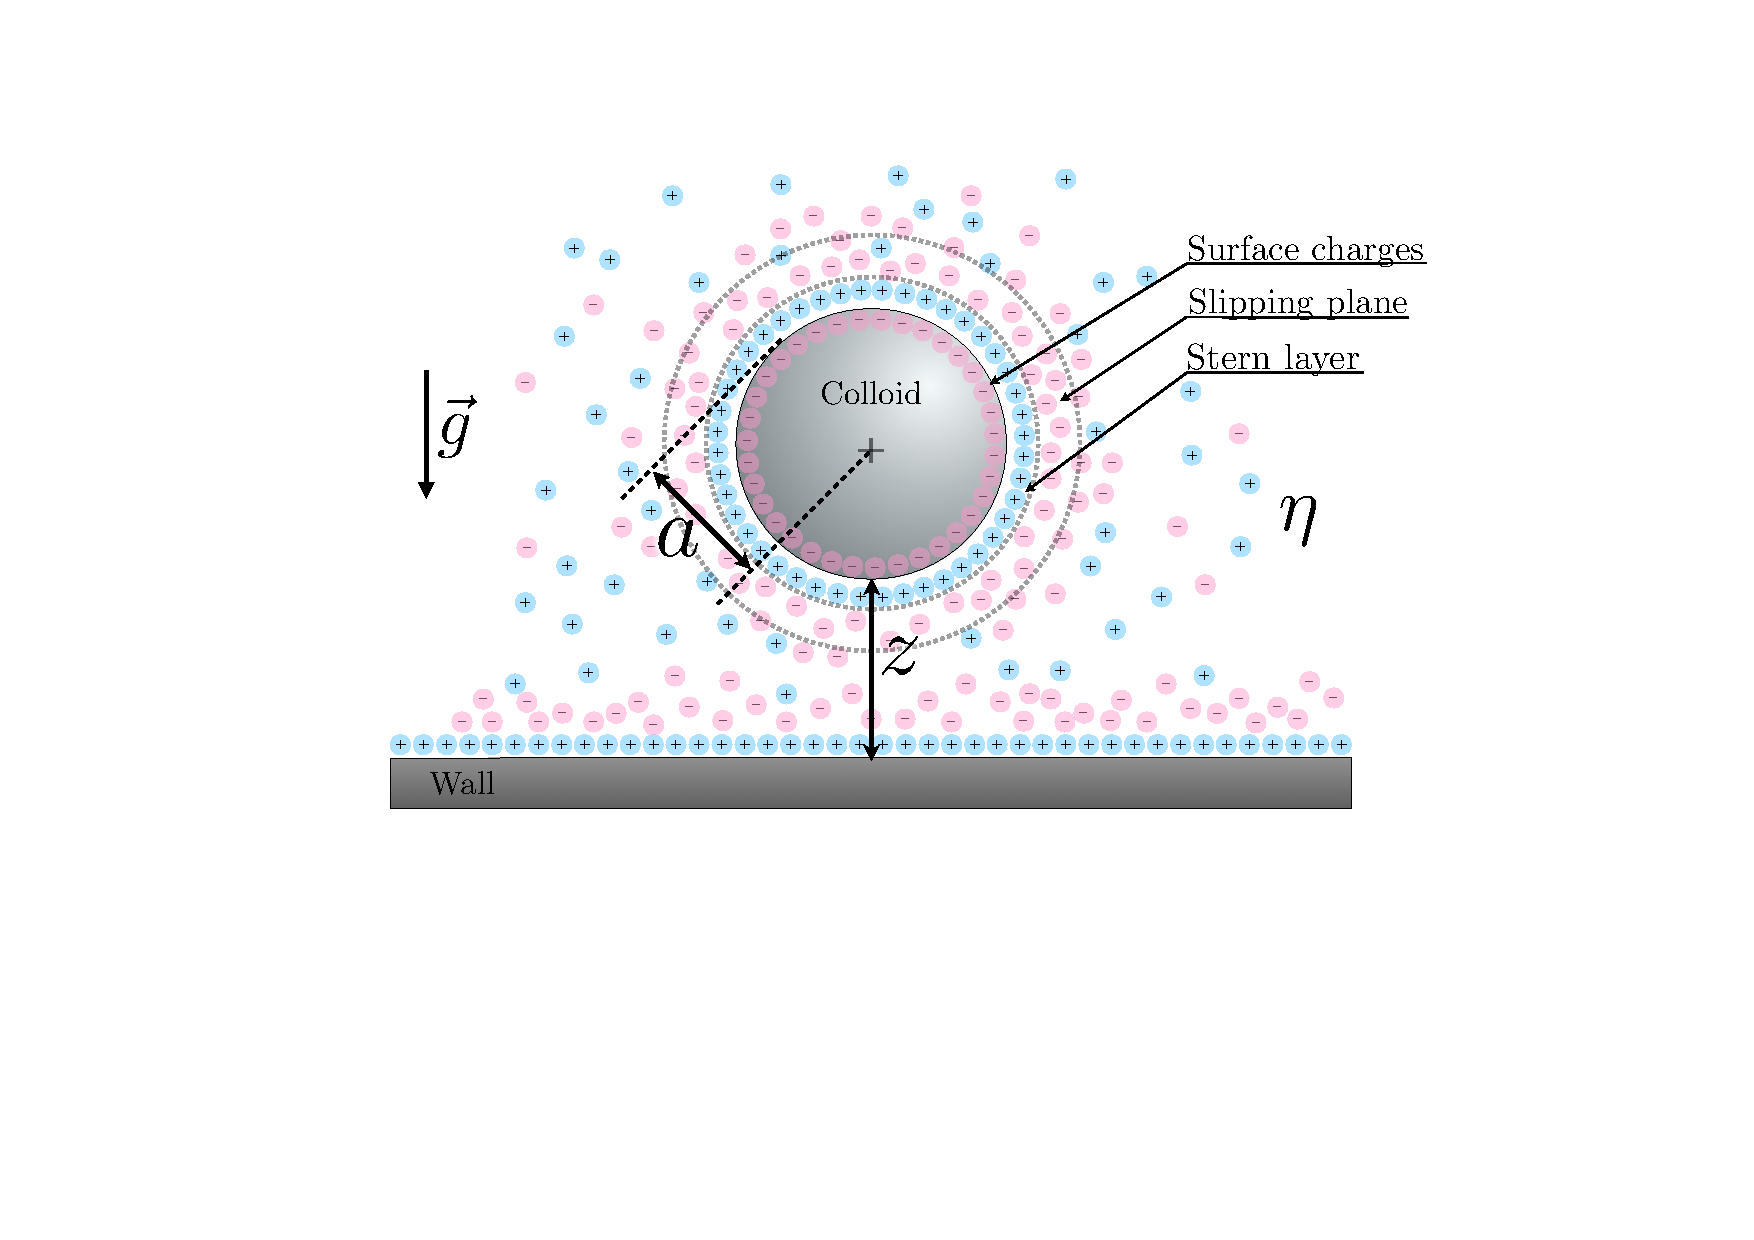
\includegraphics[width=0.8\textwidth]{figures/chapter2/double_layer.pdf}
    \caption[Schematic representation of electrostatic interactions for a silica bead immersed in salted water near a silica wall.]{Schematic representation of a colloid of radius $a$ at a distance $z$ from an infinite plane. Both surfaces are charged, and thus, a double layer of counter-ions forms around each of them.}
    \label{double_layer}
\end{figure}
Because of the amphoteric nature of silica, both the infinite place and the colloid surfaces are able to ionise when in contact with water (Fig.~\ref{double_layer}). The surfaces themselves become negatively charged, which in turn attract adsorb ions in contact with the surface, in a dense and tightly bound Stern layer. Around this plane, a mobile, ionic "atmosphere" screens the electric potential of the colloid over distance with a characteristic length $l_\mathrm{D}$, for which we provide the derivation below.
This diffuse layer, existing for both surfaces at play in the system, is responsible for the electrostatic repulsion between the two bodies (plane and colloid). It is also worth mentioning, for the sake of the following derivation of the electronic interaction potential, that within the diffuse layer exists the so-called Slipping plane. This plane separates the fluid that is dragged by the colloid from the fluid that flows around it. Experimentally speaking, this is where one measures the electrostatic potential of a surface, the $\zeta$ potential. At thermodynamic equilibrium, the local ion concentration in the diffuse layer $c_i(\vect{r})$ of a given species should follow the Boltzmann distribution:
\begin{equation}
c_i(\vect{r}) = c^\infty_{i} \exp\left\{-\dfrac{z_i e \psi(\vect{r})}{k_\mathrm{B} \Theta}\right\}~, 
\label{Boltzmann_ion_concentration}
\end{equation}
where $c_{i, \infty}$ is the bulk or infinitely far from surfaces ion concentration, $z_i$ is the valence of the ion, $e$ is the elementary charge, and $\psi(\vect{r})$ is the electrostatic potential at position $\vect{r}$, which satisfies the Poisson equation:
\begin{equation}
\nabla^2 \psi(\vect{r}) = - \dfrac{1}{\varepsilon} \sum_i z_i e c_i(\vect{r})~,
\label{poisson_equation}
\end{equation}
where $\varepsilon$ is the permittivity of the fluid. Substituting the Boltzmann distribution for $c_i(\vect{r})$ into the Poisson equation yields the Poisson-Boltzmann equation, which is a non-linear partial differential equation for $\psi(\vect{r})$. Thus, combining the above expressions, we get:
\begin{equation}
    \nabla^2 \psi(\vect{r}) + \dfrac{e}{\varepsilon} \sum_i z_i c^\infty_i \exp \left\{\dfrac{-z_i e \psi(\vect{r})}{k_\mathrm{B} \Theta} \right\} = 0~.
    \label{Psi_full_equation}
\end{equation}
We only draw our interest to sufficiently dilute solutions in terms of electrolyte concentration $[NaCl]$. In that case, we may Taylor expand the exponential term to obtain:
\begin{equation}
    \nabla^2 \psi(\vect{r}) + \dfrac{e}{\varepsilon} \sum_i z_i c^\infty_i  \left(1 - \dfrac{z_i e \psi(\vect{r})}{k_\mathrm{B} \Theta} \right) = 0~.
    \label{Psi_taylor_expanded}
\end{equation}
Since the fluid is electrically neutral,
\begin{equation}
    \sum_i z_ic^\infty_i = 0~.
\end{equation}
Thus, Eq.~\ref{Psi_taylor_expanded} becomes: 
\begin{align}
    \nabla^2 \psi(\vect{r}) &= \left[\sum_i \dfrac{z_i^2e^2c^\infty_i}{\varepsilon k_\mathrm{B} \Theta}\right] \psi(\vect{r})\\
    & = \dfrac{1}{l_\mathrm{D}} \psi(\vect{r})~,
    \label{lD_psi}
\end{align}
where $l_\mathrm{D}$ is Debye's length, as:
\begin{equation}
l_\mathrm{D} = \sqrt{\sum_i \dfrac{\varepsilon k_\mathrm{B} \Theta}{z^2_i e^2 c^\infty_i}}~.
\label{debye_length}
\end{equation}
The above expression can be used to compute the Debye length in a given solution. For the case of a monovalent salt in water, we may keep in mind the simple relation $l_\mathrm{D} = 0.304 \sqrt{C}^{-1}$, with C the salt concentration in solution.

Now, we compute the electrostatic repulsion potential between a sphere and a plane. To do so, it is convenient to consider the plane as a sphere of infinite radius, thus reducing the problem to a sphere-sphere interaction. The Debye--Huckel expression for the electrostatic potential around a single charged sphere is given in spherical coordinates by: 
\begin{equation}
\dfrac{1}{r^2}\left[ \dfrac{\partial}{\partial r} \left( r^2 \dfrac{\partial \psi(r)}{\partial r}\right) \right] = \dfrac{1}{l_\mathrm{D}^2}\psi(r)~.
    \label{spherical_debye-huckel}
\end{equation}
This equation has general solution:
\begin{equation}
    \psi(r) = K_1 \dfrac{\exp(\dfrac{r}{l_\mathrm{D}})}{r} + K_2 \dfrac{\exp(\dfrac{-r}{l_\mathrm{D}})}{r}~.
\end{equation}
Taking into account that $\lim_{r \to \infty}\psi(r) = 0$, we identify $K_1 = 0$. Thus, we can write:
\begin{equation}
    \psi(r) = K_2 \dfrac{\exp(\dfrac{-r}{l_\mathrm{D}})}{r}~.
\end{equation}
We now are left with the identification of $K_2$. To do so, we use Gauss's flux theorem, and we finally get:
\begin{equation}
    \psi(r) = \dfrac{\sigma a^2}{\varepsilon} \dfrac{\exp(\dfrac{a}{l_\mathrm{D}})}{1 + \dfrac{a}{l_\mathrm{D}}} \dfrac{\exp\left(\dfrac{-r}{l_\mathrm{D}}\right)}{r}~,
\end{equation}
where $\sigma$ is the charge density at the surface of the sphere, $a$ is its radius. Now that we have the electrostatic potential around a single sphere, we can suppose that the potential between two spheres is simply additive by approximation:
\begin{equation}
    \psi_\mathrm{tot} (r) = \psi_1(r) + \psi_2(r)~,
\end{equation}
and, with $r = a_1 + a_2 + z$ along sphere line of centers and keeping in mind cylindrical symmetry, the total electrostatic interaction potential along the z-direction becomes:
\begin{equation}
 U_\mathrm{tot}(z) = \dfrac{4\pi}{\varepsilon}\left(\dfrac{\sigma_1a_1^2}{1 + l_\mathrm{D}^{-1}a_1}\right)\left(\dfrac{\sigma_2a_2^2}{1 + l_\mathrm{D}^{-1}a_2}\right) \dfrac{\exp(-l_\mathrm{D}^{-1}z)}{a_1 + a_2 + z}~.
\end{equation}
We now have the expression of the interaction potential between two charged spheres. As stated above, we may set one of the two radii to infinity and work with this limit to obtain the interaction potential between a sphere and a plane, as:
\begin{equation}
\dfrac{U_\mathrm{elec}}{k_\mathrm{B}\Theta} = B e^{-\dfrac{z}{l_\mathrm{D}}}~,
\label{Sphere-Wall interaction}
\end{equation}
where:
\begin{equation}
    B = \dfrac{4 \pi}{k_\mathrm{B} \Theta \varepsilon}\left( \dfrac{\sigma a^2}{1 + l_\mathrm{D}^{-1} a}\right) l_\mathrm{D} \sigma_\mathrm{wall}~.
\end{equation}
We furthermore neglect the attractive Van der Waals interactions, which in our cases of study only play a role within a few nanometers, whereas the repulsive interactions take place up to a few tens of nanometers.


\subsubsection{Equilibrium distribution}
The total potential to which the colloid is subjected when immersed in water above a charged plane is expressed as:
\begin{equation}
    U(z) = U_\mathrm{g} + U_\mathrm{elec}~,
    \label{total_potentials}
\end{equation}
or, more in detail:
\begin{equation}
    \dfrac{U(z)}{k_\mathrm{B} \Theta} = B \mathrm{e}^{\dfrac{-z}{l_\mathrm{D}}} + \dfrac{z}{l_\mathrm{B}}~, ~~~~~~\forall z>0~,
    \label{total_potential_renormalised}
\end{equation}
as we do not allow the colloid to cross the boundary.

The probability to find the colloid at position $z$ given its diffusive behaviour, the gravitational and electrostatic potentials, should follow the Gibbs-Boltzmann equilibrium distribution~\cite{Boltzmann1896}:
\begin{equation}
    P_\mathrm{eq} = \dfrac{1}{Z} \exp \left( - \dfrac{U(z)}{k_\mathrm{B} \Theta} \right)~,
\end{equation}
where 1/$Z$ is a normalising factor. It is particularly useful to keep the shape of it in mind when designing a simulation, as depending on the effect one wants to probe (very dense suspension, monolayer, or inversely, virtually unbounded colloids in the $z$-plane), we may play with the parameters to get the desired behaviour.






\subsubsection{Spurious drift}
In order to reach the correct equilibrium distribution, we must derive from the correct Fokker--Planck equation the corresponding Langevin equation. Indeed, the vertical coordinate Langevin equation acquires multiplicative noise; the noise amplitude along the $z$ coordinate depends on the $z$ position itself. We begin this derivation with the general expression of the Langevin process:
\begin{equation}
    \mathrm{d}z = \dfrac{F(z)}{\gamma_\perp(z)}\mathrm{d}t + \sqrt{2D_\perp(z)}\mathrm{d}W_t~.
    \label{confinedLangevin_stochdrift}
\end{equation}
where $F(z)/\gamma_\perp(z)$ is our term of interest for the equilibrium to be conserved. We take the steady-state of Eq.~\ref{eq:fokker_planck_general}:
\begin{equation}
\dfrac{\mathrm{d}}{\mathrm{d}z} \left\{-u(z) + \dfrac{1}{2} \dfrac{\mathrm{d}}{\mathrm{d}z} g(z)^2 \right\} P_\mathrm{ss}(z) = 0~,
\end{equation}
with $u(z) = F(z)/\gamma_\perp(z)$. Because $\lim_{z\to \infty} P_\mathrm{ss}(z) = 0$ and $\lim_{z\to \infty} (\mathrm{d} P_\mathrm{ss}(z)/\mathrm{d}z) = 0$,
\begin{equation}
u(z) P_\mathrm{ss}(z) - \dfrac{1}{2} \dfrac{\mathrm{d} }{\mathrm{d} z} \left\{g(z)^2 P_\mathrm{ss}(z)\right\} = 0~.
\end{equation}
Substitute $A(z) = g^2(z)P_\mathrm{ss}(z)$:
\begin{equation}
    \dfrac{\mathrm{d}A(z)}{\mathrm{d}z} - 2\dfrac{u(z)}{g^2(z)}A(z) = 0~,
\end{equation}
which integrates as:
\begin{align}
    \ln \left(A(z)\right) &= \ln \left(g^2(z)\right) + \ln \left(P_\mathrm{ss}\right)\\
    &= \int \dfrac{u(z')}{g^2(z')/2} \mathrm{d}z'~.
\end{align}
Thus,
\begin{equation}
    P_\mathrm{ss}(z) = \dfrac{1}{g^2(z)} \exp\left[ 2 \int_0^z \dfrac{u(z')}{g^2(z')} \mathrm{d}z' \right]~.
\end{equation}
With:
\begin{equation}
\ln \left(g^2(z)\right) = \int \dfrac{2g'(z')g(z')}{g^2(z')}\mathrm{d}z'~,
\end{equation}
we get:
\begin{equation}
    U_\mathrm{ss}(z) = -k_\mathrm{B}\Theta \int\dfrac{u(z') - g(z')g'(z')}{g^2(z')/2} \mathrm{d}z'~.
\end{equation}
And, recalling that $F_\mathrm{ss} = -\mathrm{d}U_\mathrm{ss}/\mathrm{d}z$, we find:
\begin{equation}
\dfrac{F_\mathrm{ss}}{\gamma_\perp(z)} = \dfrac{F(z)}{\gamma_\perp(z)} - g(z)g'(z)~.
\end{equation}
The mean velocity derives from Eq.~\ref{confinedLangevin_stochdrift} as:
\begin{equation}
\left<\dfrac{\Delta z}{\Delta t}\right> \equiv \bar{v_\mathrm{d}} = \dfrac{F(z)}{\gamma_\perp(z)}~.
\label{avg_velocity_stochdrift}
\end{equation}
Then:
\begin{equation}
    \bar{v_\mathrm{d}} = \dfrac{1}{\gamma_\perp(z)} \dfrac{\mathrm{d}U_\mathrm{ss}(z)}{\mathrm{d}z} + \dfrac{\mathrm{d}D_\perp(z)}{\mathrm{d}z}~.
\end{equation}
We recover the deterministic drift velocity $v_\mathrm{d}$:
\begin{equation}
    \boxed{
v_\mathrm{d} = \dfrac{k_\mathrm{B}\Theta}{\gamma_\perp(z)} \left[-\dfrac{1}{l_\mathrm{D}}B \exp \left(-\dfrac{z}{l_\mathrm{D}}\right) + \dfrac{1}{l_\mathrm{B}} \right]~,}
\end{equation}
whereas the spurious drift $v_\mathrm{s}$, in the Padé approximation, reads:
\begin{equation}
    \boxed{
v_\mathrm{s} = 2D_0a\dfrac{2a^2 + 12 az + 21 z^2}{(2a^2 + 9az + z^2)^2}~.}
\label{final_stochastic_drift}
\end{equation}

Finally, the overdamped Langevin equations for confined Brownian motion read:
\begin{align}
    \mathrm{d}x &=  \sqrt{2D_\parallel(z)}\mathrm{d}W_t~,\\
    \mathrm{d}z &= \bar{v_\mathrm{d}}\mathrm{d}t +\sqrt{2D_\perp(z)}\mathrm{d}W_t~.
    \label{Eq:ODconf_langevin}
\end{align} 



\section{Colloids in hydrodynamic interaction}
We define in chapter~\ref{ch:4} the notion of Reynolds number more in detail. Herein, we work in the low-Reynolds number regime. In short, it means that a colloid does not carry inertia, but it transmits forces and stresses to the surrounding fluid (Fig.~\ref{fig:stokesflow}). The overdamped deterministic force balance reads:
\begin{equation}
m \dfrac{\mathrm{d}v}{\mathrm{d}t} = 0~,
\end{equation}
which means that:
\begin{equation}
    \vect{F_\mathrm{ext}} + \vect{F_\mathrm{hydro}} = 0~,
\end{equation}
that the colloid instantly pushes back with a hydrodynamic force $\vect{F_\mathrm{hydro}}$ on the fluid when submitted to an external force $\vect{F_\mathrm{ext}}$.
In this limit, Stokes equations are linear, the velocity field generated by one forced particle can be written as a Green function. Evaluating this flow at the position of another particle gives a hydrodynamic coupling between their velocities. This coupling is encoded in the mobility tensor. At thermal equilibrium, the fluctuation–dissipation theorem then converts this mobility tensor into a diffusion tensor. Therefore, experimentally and numerically, hydrodynamic interactions appear as correlated Brownian displacements. 

\begin{figure}
    \centering
    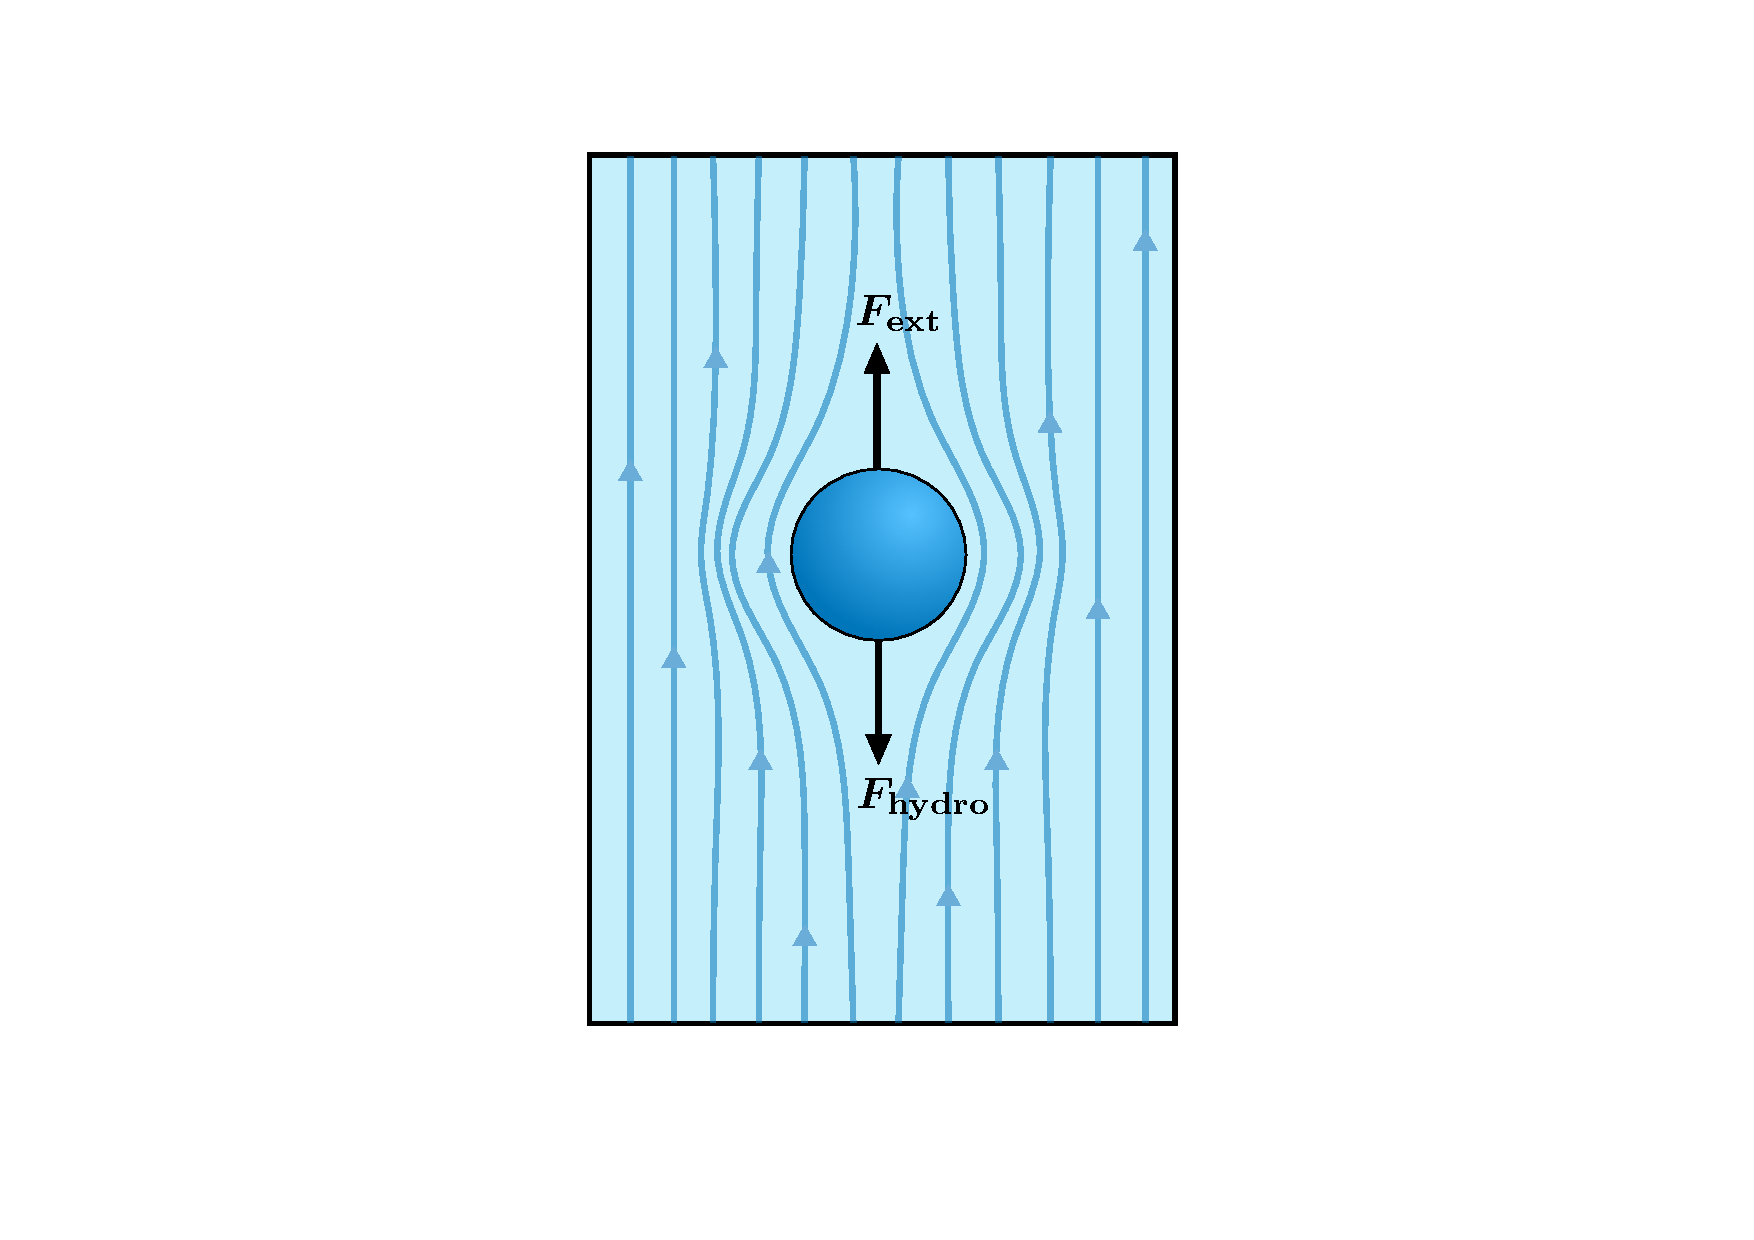
\includegraphics[width=0.3\textwidth]{figures/chapter2/stokesflow.pdf}
    \caption[Schematic of a colloid in a Stokes flow.]{Schematic of a colloid in a Stokes flow. The streamlines are represented in dark blue lines. The colloid is pushed with force $\vect{F_\mathrm{ext}}$ and pushes back on the fluid with force $\vect{F_\mathrm{hydro}}$.}
    \label{fig:stokesflow}
\end{figure}

Here, we derive under Stokes flow conditions two approximations to the mobility tensor of a colloid in hydrodynamic interaction with its neighbour. The first, called the Oseen tensor~\cite{Oseen_1927}, is shown to be typically satisfactory for colloids that are far apart ($r \gg a$). However, it supposes colloids can be approximated as point forces and neglects finite-size effects entirely~\cite{kim_microhydrodynamics_2005}. The second approximation builds on the first one and incorporates finite-size corrections for shorter inter-colloid separations. 
   
\subsection{Stokes flow, the Stokeslet and the Oseen tensor}
The Stokes equations read~\cite{happel_low_1973,kim_microhydrodynamics_2005}:
\begin{align}
    - \nabla p(\vect{r}) + \eta \nabla^2\vect{u}(\vect{r}) &= -\vect{F}\delta(\vect{r} - \vect{r_0})~,\\
    \nabla \cdot \vect{u} &= 0~, 
    \label{stokes_equations}
\end{align}
where $p$ is the pressure, $\nabla p$ is the pressure gradient in the fluid, that is to say, the force density due to pressure differences in the fluid; $\vect{r}$ is the position to origin, $\eta$ the dynamic viscosity of the fluid, $\vect{u}$ the fluid velocity field, and $\eta \nabla^2 \vect{u}$ is the viscous term that controls how the fluid diffuses momentum through itself; $\vect{F}\delta(\vect{r} - \vect{r_0})$ is the point force at $\vect{r_0}$; and the second equation denotes fluid incompressibility. Because there equations are linear, we can write the velocity response at $\vect{r}$ to a point force at $\vect{r_0}$ as a Green function~\cite{kim_microhydrodynamics_2005}:
\begin{equation}
    \vect{u}(\vect{r}) = \tens{G}(\vect{r} - \vect{r}_0) \cdot \vect{F}~.
    \label{Kim_U}
\end{equation}
This flow field generated by a point force is known as the Stokeslet flow. Then, the tensor $\tens{G}(\vect{r} - \vect{r}_0)$ is expressed:
\begin{equation}
    \tens{G(r)} = \dfrac{1}{8\pi \eta r}\left(\mat{I} + \vect{\hat{r}}\vect{\hat{r}}\right)~.
\end{equation}
The tensor $\tens{G}$ is known as the Oseen tensor~\cite{Oseen_1927}. It gives the velocity at position $\vect{r}$ induced by a \emph{point} force applied at another position. Therefore, if the particle $j$ exerts a force $\vect{F_j}$ on the fluid, the leading-order velocity induced at the position of the particle $i$ is obtained by computing this Green function at $\vect{r_i - r_j}$ (Fig.~\ref{fig:beadbead}):
\begin{equation}
    \vect{u_i} \simeq \tens{G}(\vect{r_i} - \vect{r_j}) \cdot \vect{F_j}~, \qquad i \neq j~.
\end{equation}
\begin{figure}
    \centering
    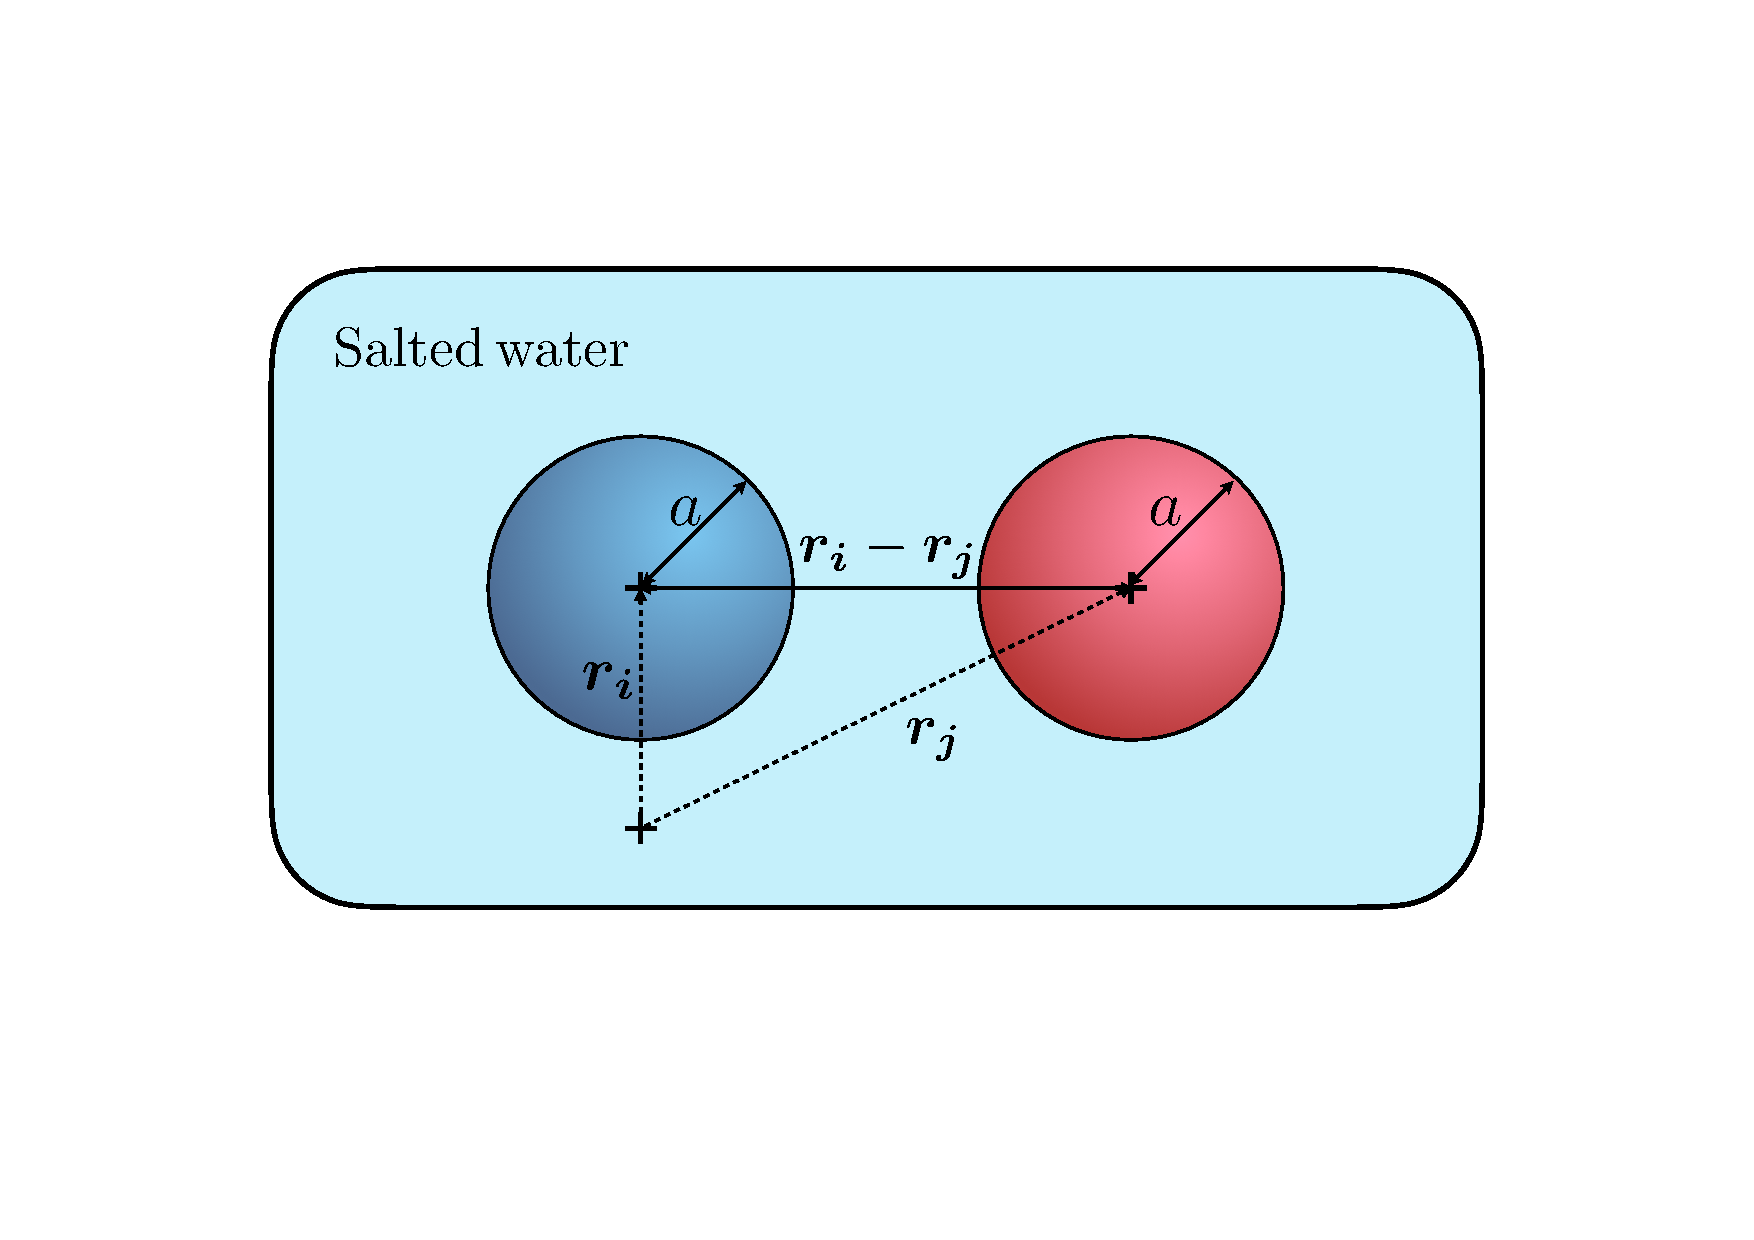
\includegraphics[width=0.6\textwidth]{figures/chapter2/beadbead.pdf}
    \caption[Two colloids interacting hydrodynamically in a bulk fluid.]{Schematic of two colloids interacting in a bulk fluid. Colloids $i$ and $j$ are at positions $\vect{r_i}$ and $\vect{r_j}$ from origin respectively, and their separation vector is denoted $\vect{r_i - r_j}$. }
    \label{fig:beadbead}
\end{figure}

\subsubsection{The mobility tensor}
The velocity field at the position of colloid $i$ generated by the other colloids in the fluid is expressed as:
\begin{equation}
\vect{u}(\vect{r}_i) =
\sum_{j\neq i}
\tens{G}(\vect{r}_i-\vect{r}_j)\cdot \vect{F}_j~,
\end{equation}
since Green's functions are linear and additive. We then express the total translational velocity $\vect{V}_i$ of colloid $i$ as:
\begin{equation}
\vect{V}_i
=
\sum_j
\tens\mu_{ij}^{tt}\cdot \vect{F}_j~,
\end{equation}
where $\tens\mu_{ij}^{tt}$ is the translational mobility block. In the Oseen approximation, it is given by:
\begin{equation}
\tens\mu_{ij}^{tt} =
\begin{cases}
\dfrac{1}{6\pi\eta a},\mat{I}~,
& i=j~, \\[1em]
\tens{G}(\vect{r}_i-\vect{r}_j)~,
& i\neq j~.
\end{cases}
\label{eq:oseen_mobility_pair}
\end{equation}
The diagonal blocks describe the self-mobility of isolated spherical colloids, while the off-diagonal blocks describe the hydrodynamic coupling between distinct colloids. The grand translational mobility matrix, regrouping all mobility blocks, is:
\begin{equation}
\mat\mu^{tt}
=
\begin{bmatrix}
\tens\mu^{tt}*{11} & \dots & \tens\mu^{tt}*{1N} \
\vdots & \ddots & \vdots \
\tens\mu^{tt}*{N1} & \dots & \tens\mu^{tt}*{NN}
\end{bmatrix}~.
\end{equation}
We focus here on translational degrees of freedom and neglect torques and rotational dynamics. The mobility tensor describes the deterministic response of the colloids to applied forces. For Brownian colloids at thermal equilibrium, the same tensor also controls the amplitude and correlations of thermal fluctuations. This connection is given by the fluctuation-dissipation theorem~\cite{einstein_uber_1905,kubo1966}:
\begin{equation}
\mat{D}^{tt}=k_\mathrm B \Theta,\mat\mu^{tt}~,
\end{equation}
where $\mat{D}^{tt}$ is the translational diffusion tensor and $k_\mathrm B\Theta$ is the thermal energy at temperature $\Theta$.

\subsubsection{Self- and cross-diffusion}

For particles $i$ and $j$, and Cartesian components $\alpha$ and $\beta$, the diffusion tensor is defined through the covariance of Brownian displacements:
\begin{equation}
\left\langle \Delta r_{i,\alpha}(\Delta t) \Delta r_{j,\beta}(\Delta t) \right\rangle = 2D^{tt}_{i\alpha,j\beta}\Delta t~.
\label{eq:cross_diffusions}
\end{equation}
The diagonal blocks, $i=j$, describe the self-diffusion of each particle, while the off-diagonal blocks, $i\neq j$, describe cross-diffusion between colloids. These off-diagonal terms quantify how Brownian displacements of distinct particles correlate through the fluid. Using the fluctuation-dissipation relation, the Oseen approximation for the translational diffusion blocks becomes:
\begin{equation}
\tens{D}_{ij}^{tt} = k_\mathrm{B}\Theta,\tens{\mu_{ij}^{tt}} =
\begin{cases}
D_0,\mat{I}~,
& i=j~, \\[1em]
k_\mathrm{B}\Theta,\tens{G}(\vect{r_i}-\vect{r_j})~,
& i \neq j~,
\end{cases}
\label{eq:oseen_diffusion_tensor_pair}
\end{equation}
where:
\begin{equation}
D_0 = \dfrac{k_\mathrm{B}\Theta}{6\pi\eta a}
\end{equation}
is the Stokes-Einstein diffusion coefficient of an isolated spherical colloid in an unbounded fluid.


\subsection{Finite-size regularisation: the Rotne-Prager-Yamakawa tensor}


By diagonalising the tensor, we retrieve
\begin{align}
 \dfrac{D^{C,R}_\perp}{2D_0}& = 1 \pm \dfrac{3}{4} \dfrac{a}{r} + \mathcal{O} \left( \dfrac{a^3}{r^3} \right)~,\\
 \dfrac{D^{C,R}_\parallel}{2D_0} &= 1 \pm \dfrac{3}{2} \dfrac{a}{r} + \mathcal{O} \left( \dfrac{a^3}{r^3} \right)~,
 \label{Oseen_dufresne_crossdifs}
\end{align}
where positive and negative corrections correspond respectively to the collective and relative modes of motion. As one may notice, hydrodynamic interactions as very long-range with respect to the colloid size and decay in $1/r$. 

\begin{figure}
     \centering
    \label{perp_para_coll_rel}
    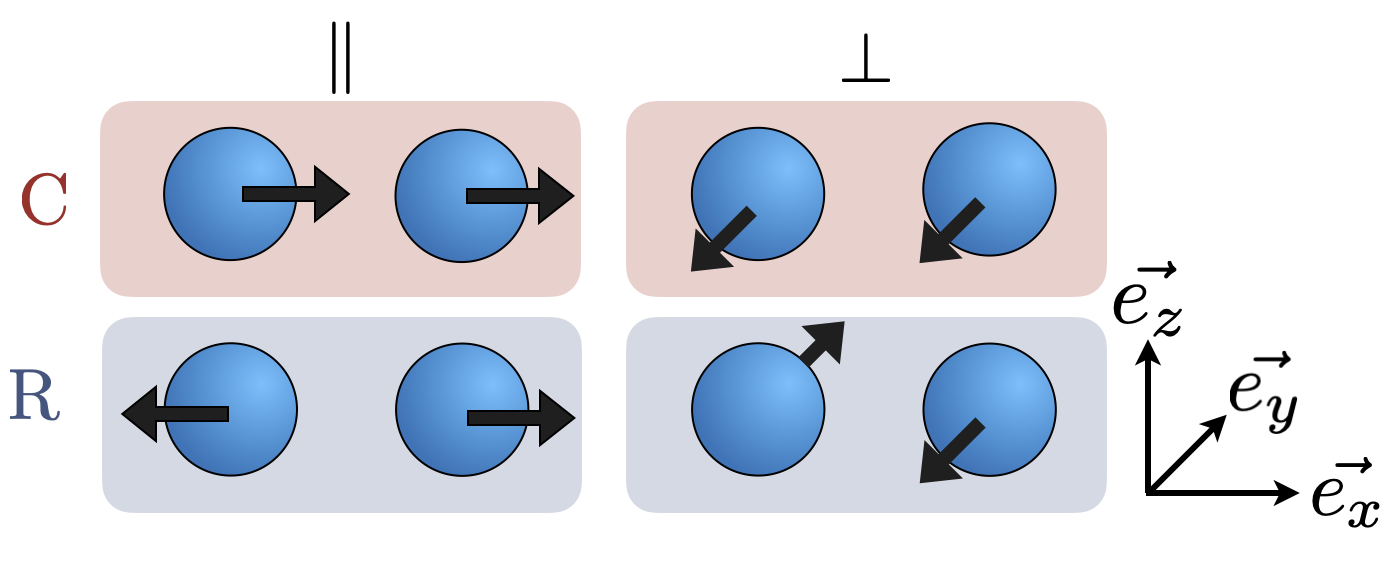
\includegraphics[width=0.8\textwidth]{figures/chapter2/collective_relative_scheme.png}
    \caption[Collective and relative cross-diffusion modes.]{Diagram of the different modes of motion of interest for two Brownian colloids. For the sake of simplicity and continuity with the rest of the chapter, we do not consider the vertical direction.}
\end{figure}


The Oseen approximation does not work for near-field interactions. Referring specifically to Eq.~\ref{Oseen_dufresne_crossdifs}, our expressions are only valid down to $r \geq 10 a$. Beyond that limit, the approximation becomes first incorrect, and then unphysical, with negative diffusion coefficients arising.

Luckily, because of its construction, the Oseen approximation is actually the first order of a more robust correction, which I detail in the next subsection.


\subsubsection{The Rotne-Prager-Yamakawa tensor}
To remedy the issues of the Oseen approximations mentioned above, we introduce the Rotne-Prager-Yamakawa (RPY) tensor, which incorporates finite size particles into the hydrodynamic interactions, at the pairwise level. This correction is, therefore, not a full N-body solution (which is anyway not solvable in a closed, analytic form, and would be a numerical nightmare to compute efficiently). I would put it, simply, as a finite-size correction to the Oseen approximation. Explicitly, for the two-colloid case,

\begin{equation}
    \tens{\mu}^{\mathrm{RPY}}_{12}(\vect{r}) = \dfrac{1}{8 \pi \eta \vect{r}} \left[ \left(1 + \dfrac{2a^2}{3r^2}\right) \mat{I} + \left(1 - \dfrac{2a^2}{r^2} \dfrac{\vect{r}\vect{r}}{r^2} \right) \right]~.
\end{equation}


This expression also ensures positive-definiteness of the mobility tensor. We will see, later down, that it is used in a modified form to account for the existence of boundaries in the fluid.

\textcolor{red}{develop.}

\section{Interactions between two colloids and a wall}
\subsection{Coupling colloid-wall and colloid-colloid lubrication theories}
Naturally, the next step is to couple both lubrication effects together. Luckily, such study has already been carried out both theoretically and experimentally by Dufresne et al. ~\cite{Dufresne_2000}. In this article, the authors discuss the modification on colloid cross-diffusion due to wall and colloid-colloid-induced lubrication effects.
The following setup, depicted in Fig. ~\ref{dufresne_system}, is used: two colloids of radius $a=0.485\pm0.025\, \upmu \mathrm{m}$ are submerged in a water-salt solution of 2mM [NaCl] and viscosity $\eta = 0.817\, \mathrm{cP}$. 
The water-salt layer is $140 \pm 2\, \upmu \mathrm{m}$ thick, and sealed between a microscope slide and a No. 1 coverslip, with the system fully sealed with UV-cured epoxy to prevent evaporation of the fluid and fluid flows in the bulk. The system is maintained at $T = 29.00 \pm 0.01 \, ^\circ \mathrm{C}$. In these conditions, the colloid self-diffusion is found to be $D_0 = k_\mathrm{B}\Theta/(6 \pi \eta a) = 0.550 \pm 0.028 \, \upmu \mathrm{m}^2/\mathrm{s}$.

\begin{figure}
    \centering
    \label{dufresne_system}
    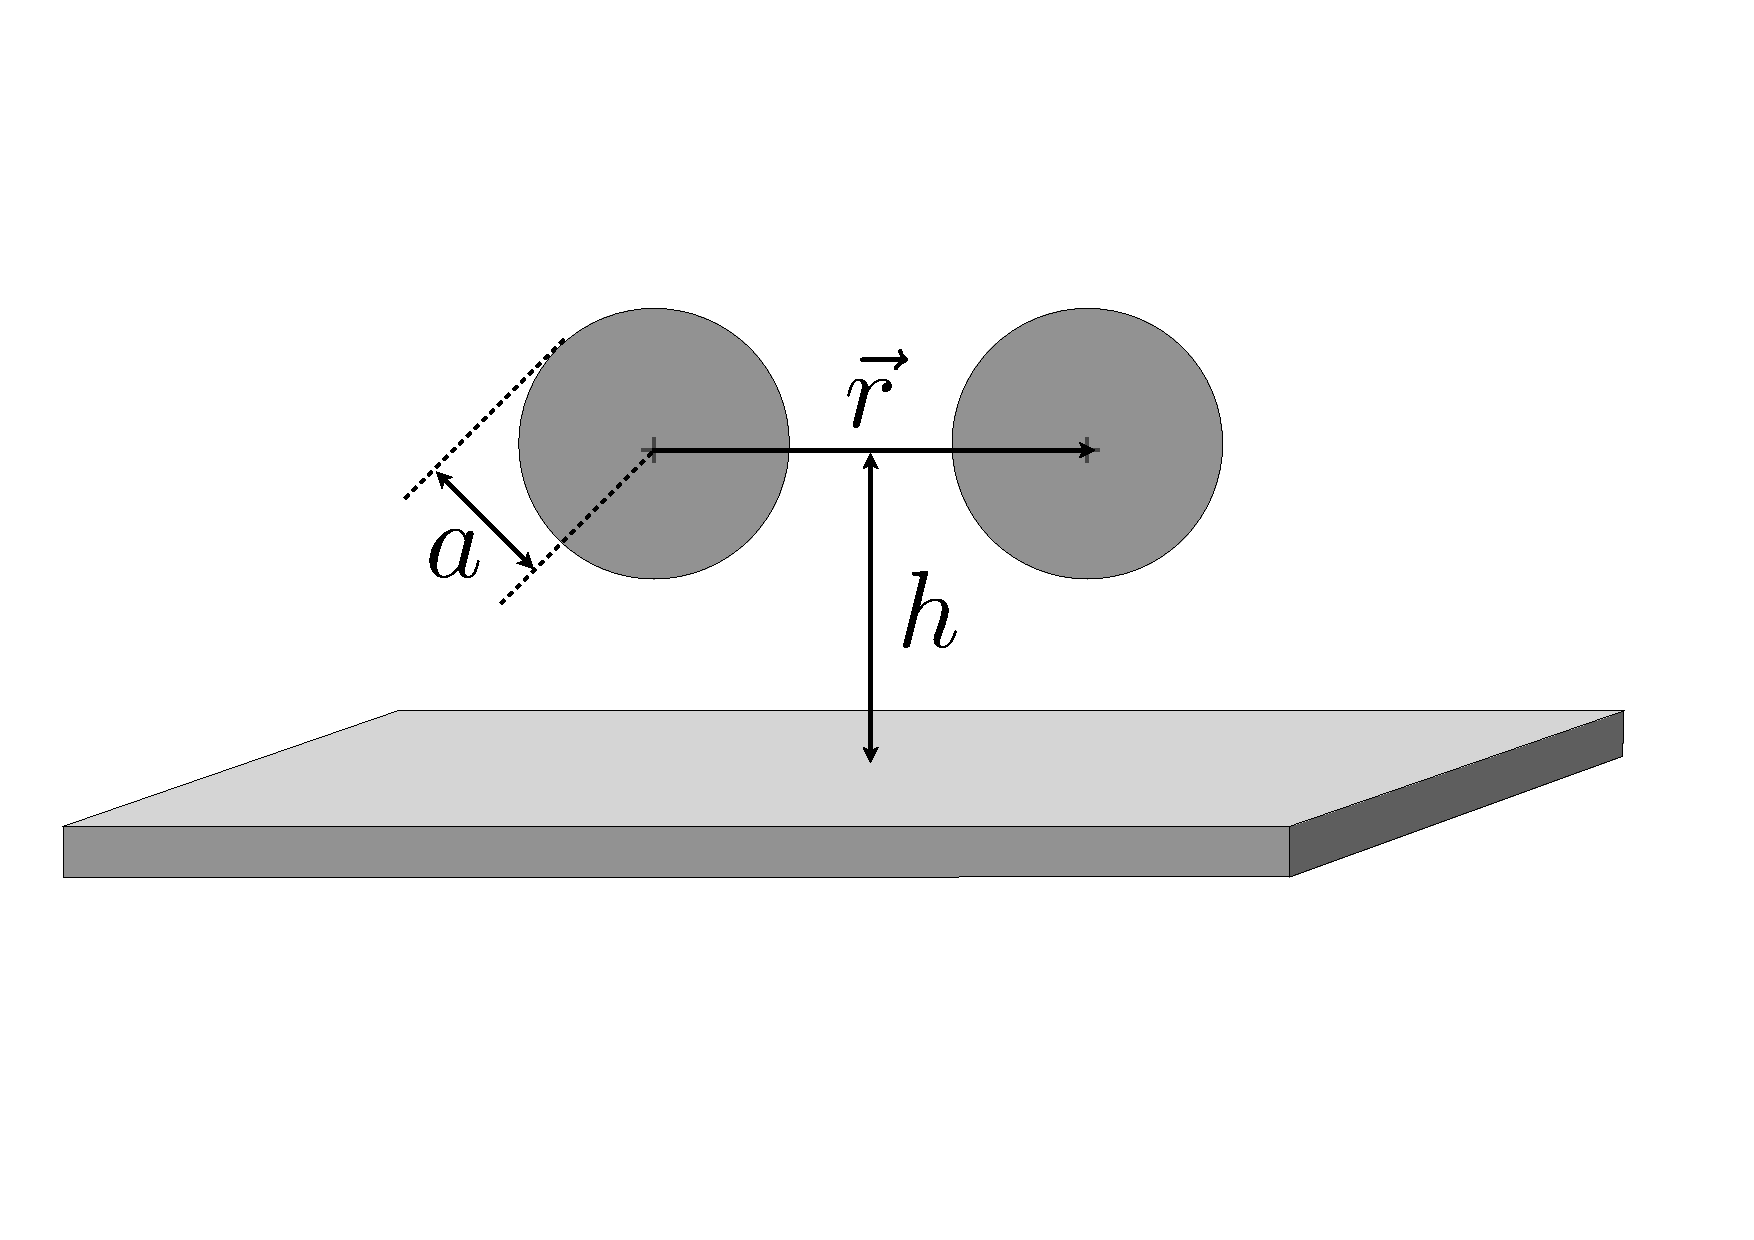
\includegraphics[width=0.8\textwidth]{figures/chapter2/dufresne_system.pdf}
    \caption[Schematic of the system studied in Dufresne \emph{et al.} ~\cite{Dufresne_2000} for colloids diffusing near each other over a wall.]{Experimental setup of Dufresne et al. ~\cite{Dufresne_2000} for the study of two colloids diffusing over a plane wall.}
\end{figure}

The authors then trap the two colloids with a single optical tweezer, by alternating the position of the focal plane at the two positions of interest at a frequency of 200Hz using a galvanometer-driven mirror. Then, by blocking the beam for $t=83\, \mathrm{ms}$, they retrieve the sphere positions over five video frames only to ensure minimal out-of-focal displacement.
From there on, authors carry out experiments over a grid of starting positions in $(r, h)$ space, with $r$ the center-to-center distance between colloids and $2\, \upmu \mathrm{m} < r < 10 \, \upmu \mathrm{m}$, and $h$ the colloid center-to-wall distance, with $1\, \upmu \mathrm{m}< h < 30\,  \upmu \mathrm{m}$.
 By reactivating the trapping, they can repeat the experiment with perfect reproducibility for each starting position of interest in their system.


As discussed in the previous sections, colloids in a same bath should see their motion coupled through hydrodynamic interactions, but the coupling to the wall itself should also modify their expected diffusion. To investigate these coupling effects, the authors decompose the trajectories of the colloids into cooperative and relative motions, respectively $\vect\rho = \vect{r_1} + \vect{r_2}$ and $\vect{r} = \vect{r_1} - \vect{r_2}$ along ($\parallel$) and perpendicular ($\perp$) directions to the line of centers of the colloids (Fig.~\ref{collective_relative_motions}). From there, they fill displacement histograms for each mode of motion at each of the five time steps taken into consideration and retrieve the effective diffusion coefficients from the standard deviation of each histogram, as:


\begin{equation}
    \langle \Delta r_{i, \alpha} ( \tau ) \Delta r_{j, \beta} \rangle = 2 D_{i\alpha, j\beta} \tau~,
\end{equation}
%%%%%%%%%%%%%%%%%%%%%%%%%%%%%%%

with $i,j \in \{1,2\}$ and $\alpha, \beta \in \{\parallel, \perp\}$, where $\tau$ is the elapsed time, and where $\langle . \rangle$ denotes an ensemble average.

A typical result of the experiment for a given set of $(r, h)$ is shown in Fig.~\ref{dufresne_results_msd}. There, MSDs are extracted from displacement histograms at each of the five time lags into consideration. From there, authors can extract the effective cross-diffusion coefficient.

\begin{figure}
    \centering
    \label{dufresne_results_msd}
    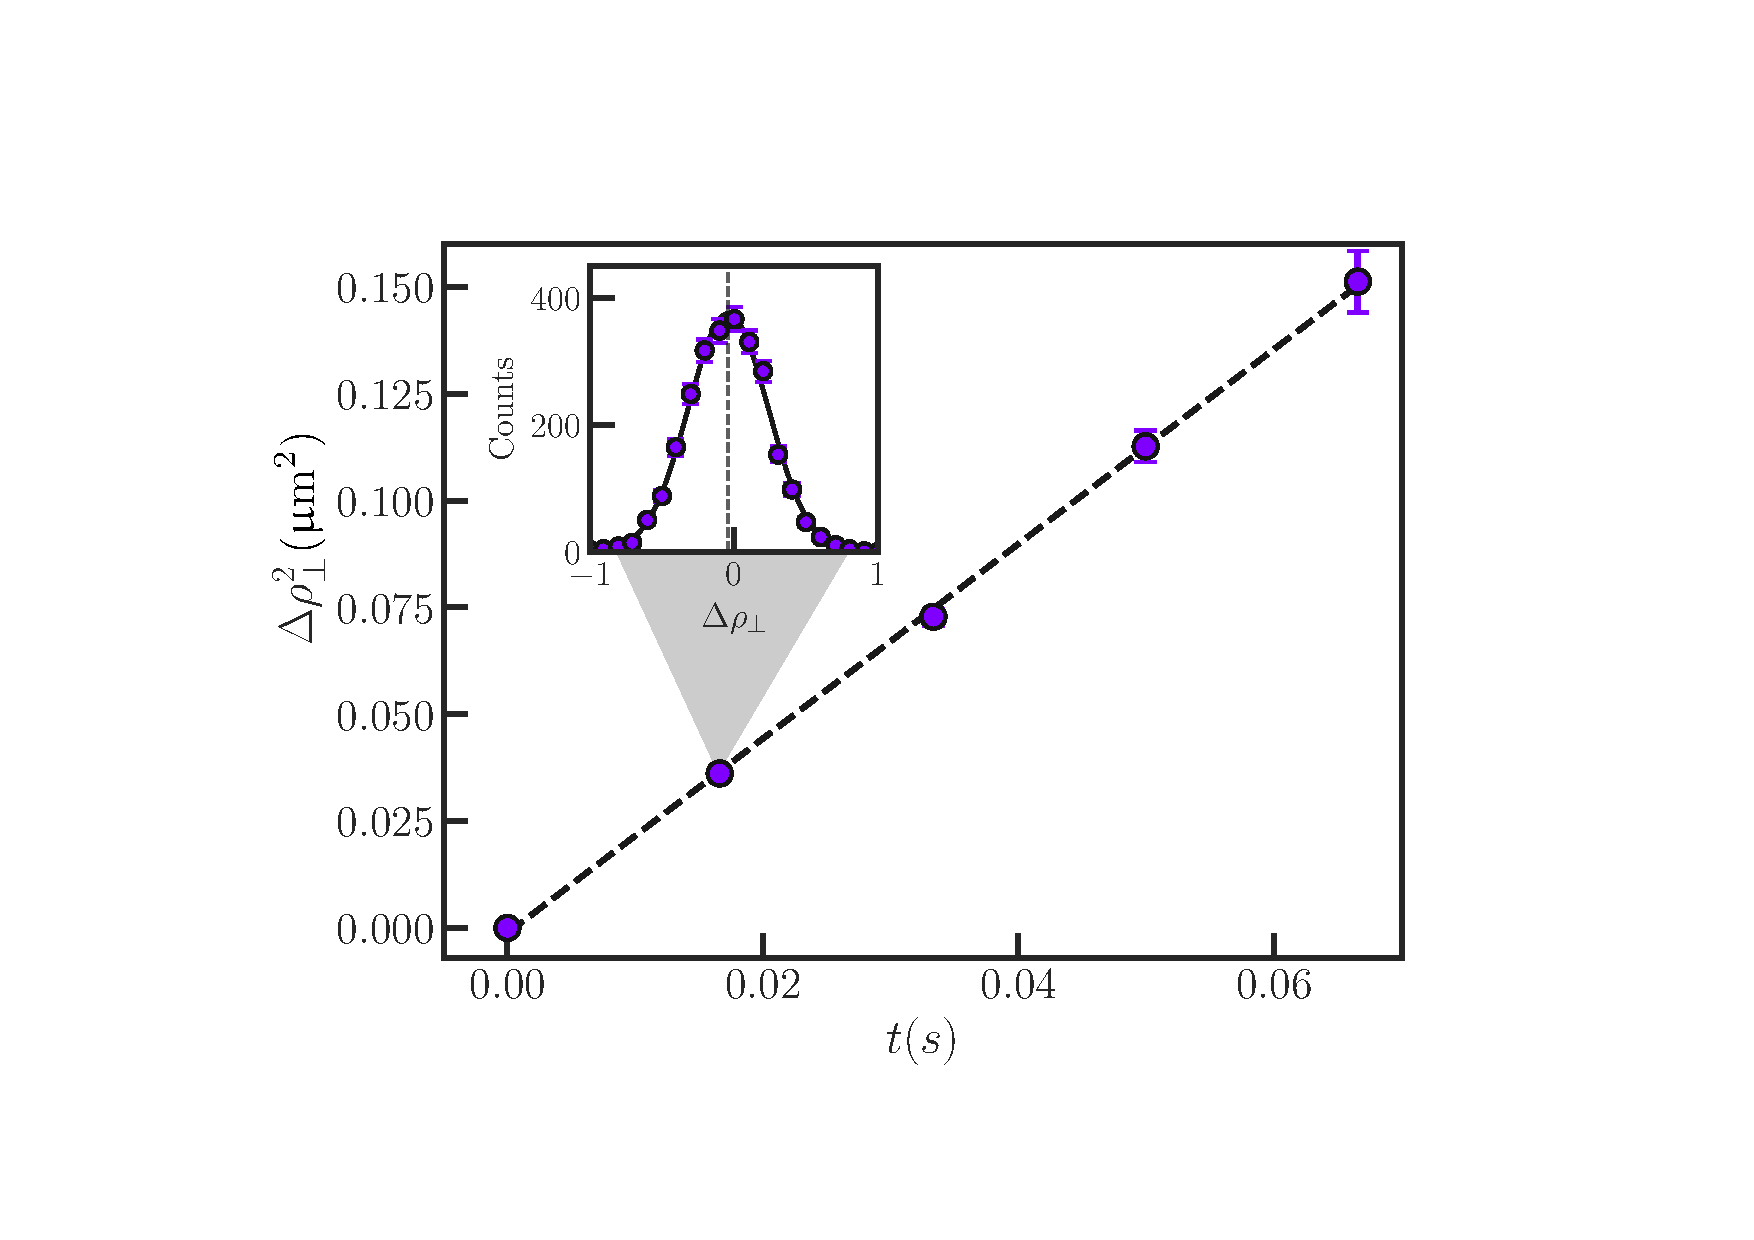
\includegraphics[width=0.8\textwidth]{figures/chapter2/dufresne_results.pdf}
    \caption[Measured pair diffusion for two colloids diffusing over a hard wall. Adapted from ~\cite{Dufresne_2000}.]{Adapted from ~\cite{Dufresne_2000}. Measured pair diffusion for the relative perpendicular mode of motion of the two colloids. The upper inset shows the histogram of all binned displacements for a given time step, for $h = 25.5\, \pm \,0.7 \upmu \mathrm{m}$ and $r = 7.00\, \pm 0.25 \upmu \mathrm{m}$. This process is repeated over all time steps and each histogram is fitted with a Gaussian curve to recover the root-mean-square displacement $\Delta \rho (r, h, \tau)$ to recover the MSD of the main plot. The effective cross-diffusion coefficient for the perpendicular mode is then extracted from the slope of the MSD.}
\end{figure}


For comparisons purposes with their experimentally retrieved cross-diffusions in the four possible modes, the authors then compute by different means the theoretical expected value of the cross-diffusion coefficients.

Now, in the presence of a wall, one must take extra care to ensure no-slip boundary conditions at the wall as well as no fluid penetration through the wall itself. To do this, one may use the single-colloid method of images ~\cite{Blake_1971}, where a Stokeslet (S), as Source Doublet (D) and a Stokeslet Doublet (SD) of opposite strength to the Stokeslet of interest at $\vect{r_j}$ above the wall is placed at equal distance below the wall, at $\vect{R_j} = \vect{r_j} - 2h \vect{e_z}$. The goal of the mirror Stokeslet is to cancel most of the normal penetration at the wall. The Source Doublet ensures no-slip at the wall, and the Stokeslet Doublet cancels remaining penetration. Then, the flow at the position of the image colloid is written:

\begin{equation}
    \label{image_system}
    G^W_{\alpha\beta} \left(\vect{x} - \vect{R_j}\right) = - G^S_{\alpha\beta}\left(\vect{x} - \vect{R_j}\right) + 2 h ^2 G^D_{\alpha\beta}\left(\vect{x} - \vect{R_j}\right) - 2 h G^{SD}_{\alpha\beta}\left(\vect{x} - \vect{R_j}\right)~,
\end{equation}

with 

\begin{align}
    \label{Image_system_details}
    G^D_{\alpha\beta} (\vect{x} - \vect{R_j}) &= \dfrac{1}{8 \pi \eta} \left( 1 - 2 \delta_{\beta z} \right) \dfrac{\partial}{\partial R_{j, \beta}} \left( \dfrac{(\vect{x} - \vect{R_j})_\alpha}{|\vect{x} - \vect{R_j}|^3} \right)~,\\
    G^{SD}_{\alpha\beta} (\vect{x} - \vect{R_j}) &= (1 - 2\delta_{\beta z}) \dfrac{\partial}{\partial R_{j, \beta}} G^S_{\alpha z} (\vect{x} - \vect{R_j})~.
\end{align}

which yields the two following modes of motion for the cross-diffusion coefficients

\begin{align}
    \label{cross_diffusion_modes}
    \dfrac{D_z}{D_0} &=   1 - \dfrac{9}{8} \dfrac{a}{r}  + \mathcal{O}\left(\dfrac{a^3}{r^3}\right)~,\\
    \dfrac{D_{xy}}{D_0} &=   1 - \dfrac{9}{16} \dfrac{a}{r} + \mathcal{O}\left(\dfrac{a^3}{r^3}\right)~.
\end{align}

One may notice the resemblance between the correction terms in the above expressions and the corrections in the Faxén formula from equation \ref{Faxén}, which is not surprising as both corrections are due to the same wall-induced hydrodynamic effects. However, these expressions are only valid in the far-field regime, and fail to capture the lubrication effects in the near-field regime, which is precisely the regime of interest for our simulations.

The authors then propose an intermediate regime, first by naively superimposing the Oseen and Blake approximations as $D_\psi^{-1}(r, h) = D_\psi^{-1}(r) + \left[D_{xy}^{-1}(h) - D_0^{-1}\right]/2$ (in dash lines in Fig.~\ref{Dufresne_cross_diffusion}), which is a crude approximation which fails to capture the behaviour of the cross-diffusion for colloids below 50 radii from the plane. The authors then propose that the colloid must interact with its image, its neighbour, and its neighbour's image. In that case, the cross-diffusion is given by

\begin{align}
\dfrac{ D^{C,R}_\perp }{ 2D_0 } &= 1 - \dfrac{9}{16} \dfrac{a}{r} \pm \dfrac{3}{4} \dfrac{a}{r} \left( 1 - \dfrac{ 1 + \dfrac{3}{2}\xi }{ (1 + \xi )^{3/2} } \right) \\
\dfrac{ D^{C,R}_\parallel }{ 2D_0 } &= 1 - \dfrac{9}{16} \dfrac{a}{r} \pm \dfrac{3}{2} \dfrac{a}{r} \left( 1 - \dfrac{1 + \xi + \dfrac{3}{2} \xi^2}{ (1 + \xi )^{5/2} }\right)
\label{cross_diffusion_modes_dufresne}
\end{align}
with $\xi = 4h^2 / r^2$ and up to $\mathcal{O} \left( a^3/r^3\right)$ and $\mathcal{O} \left( a^3/h^3\right)$ (in solid lines in Fig.~\ref{Dufresne_cross_diffusion}).


\begin{figure}
    \centering
    \label{Dufresne_cross_diffusion}
    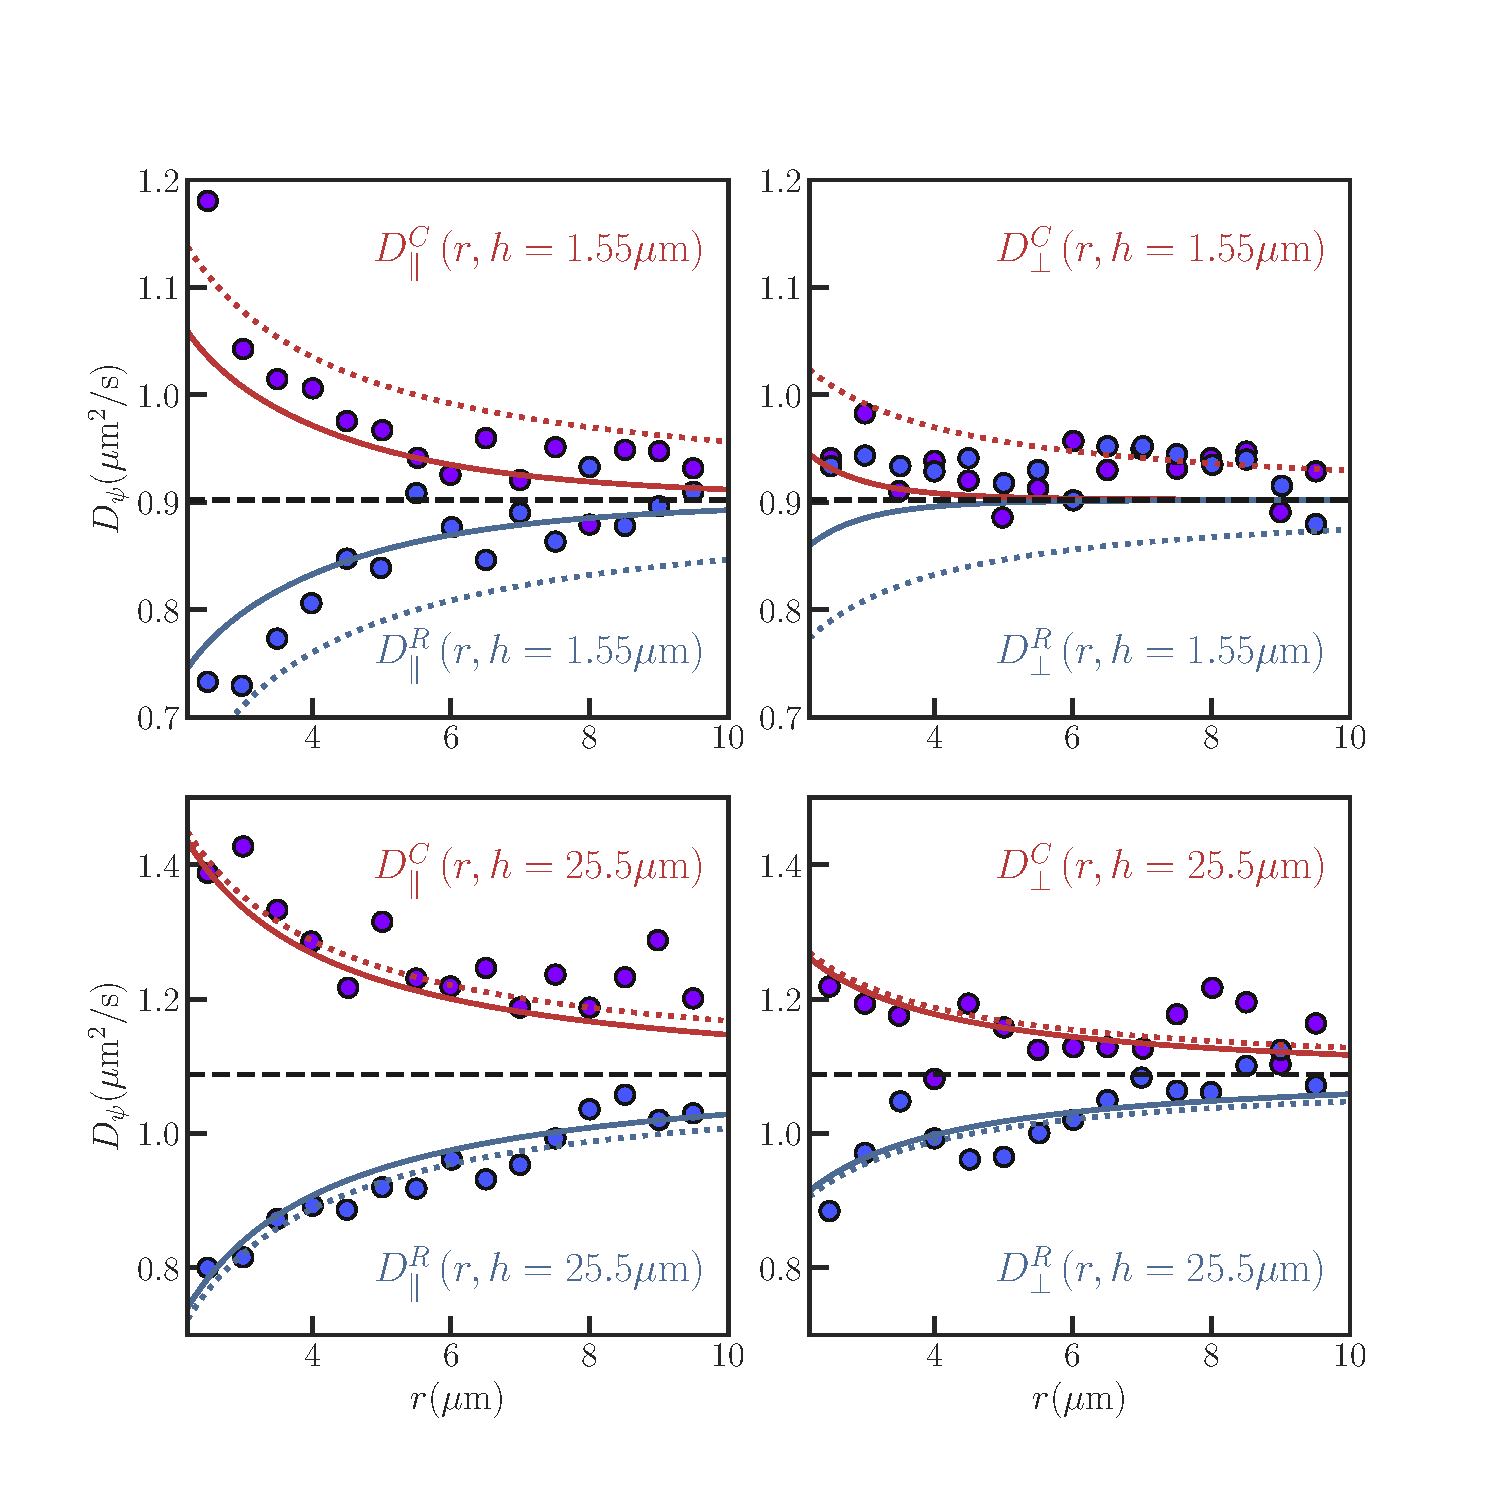
\includegraphics[width=0.8\textwidth]{figures/chapter2/dufresne_final_result.pdf}
    \caption[Measured collective and relative cross-diffusion for two colloids close to each other and near a wall, for various distances between the colloids and between the colloids' line of center and the wall. Final result from ~\cite{Dufresne_2000}.]{Adapted from ~\cite{Dufresne_2000}. Measured cross-diffusion coefficients for the relative perpendicular and parallel modes of motion of the two colloids, as a function of the center-to-center distance $r$ between the colloids, for different values of the center-to-wall distance $h$. The dash lines correspond to the naive superposition of Oseen and Blake approximations, while the solid lines correspond to the Rotne-Prager-Yamakawa \textcolor{red}{mmmh check it} approximation.}
\end{figure}


Furthermore, as noted by the authors, in the very far-field regime, the Oseen approximations should be recovered numerically and experimentally, whereas they expect the above expressions to hold in the very near-field regime as the wall hinders coupling between colloid motions. 


In the following parts, we confirm the above predictions numerically, but we push the study much deeper into the lubrication regimes to investigate its validity once we cannot ignore finite-size effects anymore in the lubrication approximations.





%%%%%%%%%%%%%%%%%%%%%%%%%%%%%%%%%%%%%%%%%%%%%%%%%%%%%%%%%%%%%%%%%%%%%%%%%%%%%%%%%%%%%%%%%%%%%%%%%%%%%%%%%%%%%%%%%%%%%%%%%%%%%%%%%%%%%%%%%%%%%%%%%%%%%%%%%%%%%%%%%%%%%%%%%%%%%%%%%%%%%%%%%%%%%%%%
\section{Simulating dense suspensions in close confinement}
Naturally, researchers have been pondering on how to simulate dense Brownian suspensions for a few decades already ~\cite{Batchelor_1976}. However, the numerical complexity of such a method (and namely, how to efficiently solve for a multiplicative noise and, a fortiori, how to compute efficiently the square root of a diffusion or mobility tensor without computational cost blowups)...

The lubrication-corrected version of the RigidMultiBlobsWall (RBW) algorithm ~\cite{sprinkle_driven_2020} \href{https://github.com/stochastichydrotools/rigidmultiblobswall}{(here on GitHub, as stochastichydrotools/rigidmultiblobswall)} aims at filling the gap  that is forbidden by the RPY approximation. As I mentioned earlier, it is computationally expensive to fully resolve the fluid and every boundary precisely. Therefore, the RBW algorithm proposes:

\begin{itemize}
    \item In the far-field, to use the RPY approximation anyway, because it is exact in that regime;
    \item In the near-field, to replace the RPY approximation by subtraction of its contribution and addition of asymptotical corrections to the mobility matrix.
\end{itemize}

In an effort of convenience, because the resistance matrix is additive, we introduce it as $\mat{R} = \mat{M}^{-1}$ the inverse of the mobility matrix.

We take again a suspension of N colloids, and enforce a no-slip boundary below on the $z=0$ plane. Formally, we write the new, corrected mobility matrix of the whole system as:

\begin{equation}
    \mat{\bar{M}} = [\mat{R} + \mat{R}^\mathrm{sup}_\mathrm{lub} - \mat{R}^\mathrm{sup}_\mathrm{RPY}]^{-1}~,
\end{equation}

where $\mat{R}$ is constructed from pairwise RPY approximations, $\mat{R}^\mathrm{sup}_\mathrm{lub}$ is the new, asymptotical corrections that are added to the resistance of nearby colloids, and $\mat{R}^\mathrm{sup}_\mathrm{RPY}$ is the erroneous RPY corrections that $\mat{R}$ includes due to the RPY not correcting the close-field appropriately.




\section{Take-home message}